\documentclass[conference]{IEEEtran}

\usepackage{amsmath,amssymb}
\usepackage{booktabs}
\usepackage{graphicx}
\usepackage{hyperref}
\usepackage{cleveref}
\usepackage{algorithm}
\usepackage{algpseudocode}
\usepackage{xcolor}
\usepackage{enumitem}
\usepackage{caption}
\usepackage{subcaption}
\usepackage{listings}
\usepackage{microtype}
\usepackage{multirow}
\usepackage{tabularx}
\usepackage{tikz}
\usepackage{pgfplots}
\pgfplotsset{compat=1.18}
\usetikzlibrary{arrows.meta,positioning,calc}
\usepackage{pifont}

\hypersetup{
  colorlinks=true,
  linkcolor=blue!70!black,
  citecolor=green!50!black,
  urlcolor=blue!60!black,
}

\lstset{
  language=Python,
  basicstyle=\ttfamily\scriptsize,
  keywordstyle=\color{blue!70!black}\bfseries,
  commentstyle=\color{green!50!black}\itshape,
  stringstyle=\color{red!60!black},
  breaklines=true,
  frame=single,
  framesep=2pt,
  rulecolor=\color{gray!40},
}

\newcommand{\ncsim}{\texttt{ncsim}}
\newcommand{\dBm}{\,\text{dBm}}
\newcommand{\dB}{\,\text{dB}}
\newcommand{\mW}{\,\text{mW}}
\newcommand{\MHz}{\,\text{MHz}}
\newcommand{\GHz}{\,\text{GHz}}
\newcommand{\Mbps}{\,\text{Mbps}}
\newcommand{\MBps}{\,\text{MB/s}}
\newcommand{\cmark}{\ding{51}}
\newcommand{\xmark}{\ding{55}}

\title{\ncsim{}: A Lightweight Discrete-Event Simulator\\for Networked Computing with 802.11 WiFi Models}
\author{
\IEEEauthorblockN{Bhaskar Krishnamachari\IEEEauthorrefmark{1},
Maya Gutierrez\IEEEauthorrefmark{1}, and
Jared Coleman\IEEEauthorrefmark{1}\IEEEauthorrefmark{2}}
\IEEEauthorblockA{\IEEEauthorrefmark{1}University of Southern California\\
bkrishna@usc.edu, mayaguti@usc.edu}
\IEEEauthorblockA{\IEEEauthorrefmark{2}Loyola Marymount University\\
jared.coleman@lmu.edu}
}

\begin{document}
\maketitle

%% ============================================================
\begin{abstract}
We present \ncsim{}, a deterministic discrete-event simulator for evaluating
task scheduling algorithms on heterogeneous networked computing systems.
\ncsim{} models directed acyclic graph (DAG) workflows, multi-hop routing
with bandwidth sharing, and IEEE~802.11 WiFi links with a
physically-grounded CSMA/CA interference model based on Bianchi's analysis,
including contention and hidden terminal SINR degradation.
The simulator supports pluggable scheduling
algorithms (including HEFT and CPOP via the SAGA library) and three routing
strategies.
Implemented in approximately 5,500 lines of Python with YAML-driven scenario
specification, \ncsim{} fills a gap between heavyweight network simulators
like ns-3 and task-centric simulators like SimGrid, enabling rapid
exploration of the interplay between compute placement and network transport
in edge and fog computing deployments.  We validate the WiFi model against
analytical predictions across nine internal experiments (all matching within
1\% tolerance) and externally against Bianchi's published results (matching
within 0.003\%).  Using \ncsim{}, we conduct a 108-run experimental study
demonstrating that ignoring wireless interference leads to not just
inaccurate makespan predictions but systematically wrong scheduler choices
in 38.9\% of scenarios, with performance regret reaching 484\%---underscoring
the need for interference-aware simulation in wireless edge computing
research.
\end{abstract}

%% ============================================================
\section{Introduction}
\label{sec:intro}

Edge and fog computing architectures distribute computation across
heterogeneous nodes connected by networks of varying capacity and
reliability~\cite{shi2016edge}.  Effective task scheduling in these
environments requires co-optimizing compute placement and network transport:
a task placement that minimizes computation time may incur excessive data
transfer costs, while a network-aware placement may underutilize fast
processors.

Existing simulation tools address parts of this problem.  Network simulators
such as ns-3~\cite{ns3} and OMNeT++~\cite{omnetpp} provide detailed protocol
stacks but are heavyweight, complex to configure, and lack native support for
DAG-based task scheduling.  Conversely, task scheduling simulators such as
SimGrid~\cite{simgrid}, WRENCH~\cite{wrench}, and CloudSim~\cite{cloudsim}
model workflows and compute resources but typically abstract the network as
point-to-point links with fixed bandwidths, omitting wireless contention,
interference, and multi-hop effects.  Edge-specific tools like
iFogSim~\cite{ifogsim} and EdgeCloudSim~\cite{edgecloudsim} add
domain-specific features but use simplified wireless models that do not
capture the distance-dependent rates, CSMA contention, or hidden terminal
interference that characterize real 802.11 deployments.

This gap matters more than one might expect.  In a 108-run experimental
study that we conduct using \ncsim{}, we find that the scheduler which
appears optimal under an interference-free model is \emph{dominated} under
realistic CSMA/CA conditions in 38.9\% of scenarios, with makespan errors
exceeding $69\times$.  The sophisticated HEFT scheduler, optimized under
a model that ignores wireless contention, can produce \emph{worse} outcomes
than a simple round-robin baseline.  These findings underscore that realistic
wireless modeling is not merely a refinement---it is essential for
meaningful evaluation of edge computing scheduling algorithms.

We present \ncsim{}, a lightweight discrete-event simulator that bridges
this gap.  \ncsim{} combines DAG workflow scheduling with
physically-grounded 802.11 WiFi models in a single, easy-to-use Python
package.  Our contributions are:

\begin{enumerate}[itemsep=2pt,leftmargin=*]
\item A modular simulation architecture with abstract base classes for
  schedulers, routing models, interference models, link models, and queue
  models, enabling pluggable experimentation.
\item An 802.11 WiFi model incorporating log-distance path loss, MCS rate
  adaptation (802.11n/ac/ax), conflict graph construction, CSMA/CA contention
  via Bianchi's analysis, and hidden terminal SINR degradation.
\item Multi-hop routing with dynamic bandwidth sharing and three routing
  strategies (direct, widest-path, shortest-path).
\item Comprehensive validation: nine internal experiments achieving exact
  match with analytical predictions, plus external validation against
  Bianchi's published results~\cite{bianchi2000} (within 0.003\%).
\item Experimental demonstration---via a 108-run scheduler comparison
  and sensitivity analyses---that interference-free models lead to
  systematically wrong scheduling decisions, motivating the need for
  tools like \ncsim{}.
\item An open-source implementation in ${\sim}5{,}500$ lines of Python with
  YAML-driven scenarios, JSONL trace output, and a React/D3 visualization
  frontend.
\end{enumerate}

The remainder of this paper is organized as follows.
\Cref{sec:related} surveys related simulators and positions \ncsim{} in the
landscape.  \Cref{sec:arch} describes the modular architecture and its design
rationale.  \Cref{sec:model} presents the system model, including the
physically-grounded WiFi equations.  \Cref{sec:engine} details the
discrete-event simulation engine.  \Cref{sec:validation} validates the WiFi
model through both internal analytical experiments and external reproduction
of Bianchi's published results.  \Cref{sec:eval} presents the experimental
evaluation, including routing comparison, interference impact analysis,
a 108-run scheduler comparison revealing rank inversions, and sensitivity
analyses.  \Cref{sec:viz} describes the visualization tooling.
\Cref{sec:discussion} discusses the implications and limitations of our
findings.  Finally, \Cref{sec:conclusion} concludes with directions for
future work.


%% ============================================================
\section{Related Work}
\label{sec:related}

In this section, we survey existing simulation tools and position \ncsim{}
relative to them.  We organize the discussion by the primary focus of each
tool class and highlight the gap that motivates our work.

\textbf{Network simulators.}
ns-3~\cite{ns3} and OMNeT++~\cite{omnetpp} provide detailed WiFi,
LTE, and TCP/IP protocol stacks with high-fidelity channel models, making
them the standard choice for protocol-level wireless research.
However, these tools are heavyweight: configuring an ns-3 scenario with
custom DAG scheduling requires integrating external workflow engines,
writing C++ glue code, and accepting simulation times that are orders of
magnitude longer than the simulated duration.  In our experience, a single
16-node scenario that \ncsim{} completes in under 2~seconds would require
several minutes in ns-3 with equivalent WiFi and application-layer setup.
This computational cost makes parameter sweeps across hundreds of
scheduler/routing/topology combinations prohibitive for researchers whose
primary interest is scheduling algorithm design rather than protocol
engineering.

\textbf{Task scheduling simulators.}
SimGrid~\cite{simgrid} and WRENCH~\cite{wrench} model distributed
computing platforms with analytical network models and support DAG
workflows natively.  CloudSim~\cite{cloudsim} targets cloud computing with
VM-level abstractions, and has been widely adopted for evaluating resource
allocation policies.  These tools model networks as links with
fixed or analytically-derived bandwidths, without wireless contention,
hidden terminal effects, or carrier-sense-based spatial reuse.  This
abstraction is appropriate for wired data center networks where bandwidth
is dedicated and predictable.  However, in wireless edge deployments, the
effective bandwidth of a link depends on which other links are
simultaneously active---a dependency that fixed-bandwidth models cannot
capture.  As we demonstrate in \Cref{sec:eval}, this omission can lead to
not merely inaccurate predictions but systematically wrong conclusions about
which scheduling algorithm is superior.

\textbf{Edge/fog-specific simulators.}
iFogSim~\cite{ifogsim} extends CloudSim for fog computing topologies,
adding latency-sensitive application placement.
EdgeCloudSim~\cite{edgecloudsim} adds mobility and simplified WLAN
models, typically using constant bandwidth with optional capacity
degradation under load.  While these tools capture some aspects of
edge deployments, their wireless models do not account for
distance-dependent rates, CSMA/CA contention dynamics, or hidden
terminal interference---the phenomena that, as we show, most strongly
affect scheduling outcomes in multi-hop wireless networks.

\textbf{Positioning of \ncsim{}.}
\ncsim{} occupies a position between these tool classes: it combines
DAG-aware task scheduling with physically-grounded 802.11 wireless models
(SNR-based MCS rate adaptation, Bianchi MAC efficiency, SINR-based hidden
terminal modeling) in a lightweight Python package.  Unlike ns-3, \ncsim{}
does not simulate packet-level protocol stacks, which keeps simulation
times tractable for large parameter sweeps.  Unlike SimGrid and WRENCH,
\ncsim{} does not abstract away wireless interference, which preserves the
scheduling-relevant effects of contention and hidden terminals.  To this
end, \ncsim{} is well-suited for rapid exploration of scheduling algorithms
in wireless edge computing scenarios where both compute placement and
wireless network effects matter.  \Cref{tab:sim_comparison} summarizes
this positioning.

\begin{table}[t]
\centering
\caption{Simulator comparison. \ncsim{} uniquely combines DAG-native
scheduling with CSMA/CA and hidden terminal modeling at flow-level
granularity.}
\label{tab:sim_comparison}
\setlength{\tabcolsep}{3.5pt}
\begin{tabular}{@{}lcccccc@{}}
\toprule
\textbf{Tool} & \rotatebox{70}{\textbf{DAG}} &
  \rotatebox{70}{\textbf{WiFi}} &
  \rotatebox{70}{\textbf{CSMA}} &
  \rotatebox{70}{\textbf{Hid.\ Term.}} &
  \rotatebox{70}{\textbf{Pkt-Level}} &
  \rotatebox{70}{\textbf{Sweep}} \\
\midrule
ns-3~\cite{ns3}          & \xmark & \cmark & \cmark & \cmark & \cmark & High \\
OMNeT++~\cite{omnetpp}   & \xmark & \cmark & \cmark & \cmark & \cmark & High \\
SimGrid~\cite{simgrid}   & \cmark & \xmark & \xmark & \xmark & \xmark & Low \\
WRENCH~\cite{wrench}     & \cmark & \xmark & \xmark & \xmark & \xmark & Low \\
CloudSim~\cite{cloudsim} & \cmark & \xmark & \xmark & \xmark & \xmark & Low \\
iFogSim~\cite{ifogsim}   & \cmark & \xmark & \xmark & \xmark & \xmark & Med \\
EdgeCloudSim~\cite{edgecloudsim} & \xmark & \cmark & \xmark & \xmark & \xmark & Med \\
\textbf{\ncsim{}}        & \cmark & \cmark & \cmark & \cmark & \xmark & \textbf{Low} \\
\bottomrule
\end{tabular}
\end{table}


%% ============================================================
\section{Architecture}
\label{sec:arch}

In this section, we describe the architecture of \ncsim{}, which is organized
around a layered discrete-event simulation (DES) engine with pluggable
components for scheduling, routing, and interference modeling.
\Cref{fig:architecture} illustrates the data flow from scenario
specification through simulation to output traces.

\begin{figure}[t]
\centering
\fbox{\parbox{0.93\columnwidth}{\small
\textbf{Input:} Scenario YAML $\rightarrow$ Scenario Loader\\[3pt]
$\downarrow$\\[2pt]
\textbf{Core:} Network + DAGs + Config\\[2pt]
$\downarrow$\\[2pt]
\textbf{Simulation Engine}\\
\quad Event Queue (min-heap, 6 event types)\\
\quad Execution Engine (state machine)\\
\quad$\hookleftarrow$ Scheduler (HEFT, CPOP, RoundRobin, Manual)\\
\quad$\hookleftarrow$ Routing Model (Direct, Widest, Shortest)\\
\quad$\hookleftarrow$ Interference Model (None, CSMA Bianchi)\\[2pt]
$\downarrow$\\[2pt]
\textbf{Output:} JSONL Trace + Metrics JSON
}}
\caption{High-level architecture of \ncsim{}.}
\label{fig:architecture}
\end{figure}

\subsection{Design Goals}

The design of \ncsim{} is guided by four principles, each motivated by
the requirements of scheduling research in wireless edge computing.

\textbf{Determinism.}  Given the same scenario and random seed, \ncsim{}
produces bit-identical results across runs and platforms.  We achieve this by
rounding all floating-point simulation times to microsecond precision
($10^{-6}$\,s), which prevents the accumulation of platform-dependent
rounding errors that can reorder near-simultaneous events.  Determinism is
essential for reproducible scheduling comparisons: if two schedulers produce
makespans of 12.37\,s and 12.39\,s, the ranking must not change when the
experiment is re-run on a different machine.

\textbf{Modularity.}  Six abstract base classes (ABCs) define clean extension
points: \texttt{Scheduler}, \texttt{RoutingModel}, \texttt{InterferenceModel},
\texttt{LinkModel}, \texttt{QueueModel}, and \texttt{DAGSource}.  We chose
this design because scheduling research often requires comparing algorithms
across identical scenarios---modularity ensures that swapping a scheduler
does not require changes to the network model, and vice versa.  New
strategies can be added by implementing a single ABC without modifying the
core simulation engine.

\textbf{Simplicity.}  Scenarios are specified in YAML files that declaratively
describe the network topology, DAG workflows, and simulation parameters.
The entire simulator is implemented in approximately 5,500 lines of Python
with minimal dependencies (only the optional SAGA library for HEFT/CPOP
scheduling).  We deliberately chose Python over C++ or Java to lower the
barrier for researchers who wish to extend the simulator or inspect its
internals.

\textbf{Physical grounding.}  Wireless link bandwidths are derived from RF
parameters (transmit power, frequency, path loss exponent) rather than
specified as arbitrary constants.  This ensures that link rates are
physically consistent with node positions---a property that is essential
for meaningful interference modeling, since contention and hidden terminal
effects depend on the spatial relationships among transmitters and receivers.

\subsection{Design Trade-offs}

\ncsim{} intentionally omits several features to maintain its lightweight,
fast character while retaining the key phenomena---contention, hidden
terminals, MCS adaptation---that affect scheduling decisions:

\begin{itemize}[itemsep=1pt,leftmargin=*]
\item \textbf{No packet-level simulation.}  There is no TCP/IP stack or
  per-packet event processing; transfers are modeled as bulk flows with
  analytically-derived rates.
\item \textbf{No physical-layer channel dynamics.}  Fading, OFDM subcarrier
  allocation, and time-varying channel states are not modeled; path loss is
  static and deterministic (with optional log-normal shadow fading).
\item \textbf{No mobility.}  The topology is static; node positions are fixed
  for the duration of a simulation run.
\item \textbf{Single-slot compute.}  Each node executes one task at a time
  (FIFO queuing); GPU-like multi-slot parallelism is left to future work.
\end{itemize}

\noindent These choices keep simulation runtimes on the order of seconds for
networks of up to 16 nodes and 20-task DAGs, enabling rapid parameter sweeps
that would be infeasible with packet-level simulators.
\Cref{tab:scope} further summarizes the phenomena modeled and the boundaries
of validity.

\begin{table}[t]
\centering
\caption{Scope of validity: phenomena modeled by \ncsim{} and their
impact on scheduling studies.}
\label{tab:scope}
\begin{tabular}{@{}lll@{}}
\toprule
\textbf{Phenomenon} & \textbf{Status} & \textbf{Impact} \\
\midrule
CSMA/CA contention    & Modeled (Bianchi)       & High \\
Hidden terminals      & Modeled (SINR)          & High \\
MCS rate adaptation   & Modeled (11n/ac/ax)     & Medium \\
Path loss             & Modeled (log-distance)  & High \\
Pkt-level dynamics    & Not modeled             & Low$^\dagger$ \\
TCP slow-start        & Not modeled             & Medium$^\ddagger$ \\
Fading / mobility     & Optional (log-normal)   & Low$^\S$ \\
Multi-slot parallelism & Not modeled            & App-dependent \\
\bottomrule
\multicolumn{3}{@{}l}{\scriptsize $^\dagger$For bulk transfers.
  $^\ddagger$For short flows. $^\S$For static deployments.}
\end{tabular}
\end{table}

\subsection{Key Abstractions}

\Cref{tab:abstractions} summarizes the six pluggable abstractions in \ncsim{}.

\begin{table}[t]
\centering
\caption{Pluggable abstractions in \ncsim{}.}
\label{tab:abstractions}
\begin{tabular}{@{}lp{4.8cm}@{}}
\toprule
\textbf{ABC} & \textbf{Implementations} \\
\midrule
Scheduler & Manual, RoundRobin, HEFT, CPOP \\
RoutingModel & Direct, WidestPath, ShortestPath \\
InterferenceModel & None, CSMA Bianchi \\
LinkModel & Static (future: position-based, TDMA) \\
QueueModel & FIFO (future: priority, multi-slot) \\
DAGSource & Single, Multi \\
\bottomrule
\end{tabular}
\end{table}


%% ============================================================
\section{System Model}
\label{sec:model}

In this section, we present the formal models underlying \ncsim{}: the
network and compute infrastructure, the DAG workflow representation,
the scheduling and routing frameworks, and the physically-grounded
802.11 WiFi model that captures contention and hidden terminal effects.

\subsection{Network Model}

A network consists of \emph{nodes} and directed \emph{links}.  Each node $v$
has a compute capacity $C_v$ (compute units per second) and an optional 2D
position $(x_v, y_v)$ used for RF calculations.  Each link $\ell$ from node
$u$ to node $v$ has a bandwidth $B_\ell$ (MB/s) and latency $L_\ell$
(seconds).  Topologies are specified in YAML and can be arbitrary directed
graphs.

\subsection{Compute Model}

A task $t$ has a compute cost $w_t$ (in compute units).  The execution time
on node $v$ is $w_t / C_v$.  Each node processes one task at a time using
FIFO queuing.  Tasks follow a five-state lifecycle: \textsc{Pending}
$\rightarrow$ \textsc{Ready} $\rightarrow$ \textsc{Queued} $\rightarrow$
\textsc{Running} $\rightarrow$ \textsc{Completed}.

\subsection{DAG Workflow Model}

Workflows are modeled as directed acyclic graphs (DAGs) where nodes represent
tasks and edges represent data dependencies.  Each edge $e = (t_i, t_j)$
carries a data payload of size $d_e$ (in MB) that must be transferred from
the node executing $t_i$ to the node executing $t_j$ before $t_j$ can begin.
If $t_i$ and $t_j$ are placed on the same node, the transfer is
instantaneous (zero cost).  DAGs are injected at specified simulation times.

\subsection{Scheduling Framework}

The scheduler receives a \texttt{NetworkSnapshot}---an immutable view of
node capacities, link bandwidths, queue depths, and active transfers---and
returns a \texttt{PlacementPlan} mapping each task to a node.  \ncsim{}
includes four schedulers:

\begin{itemize}[itemsep=1pt,leftmargin=*]
\item \textbf{Manual:} Uses \texttt{pinned\_to} annotations from the YAML.
\item \textbf{RoundRobin:} Cycles through nodes, respecting pin constraints.
\item \textbf{HEFT/CPOP:} Adapted from the SAGA scheduling library~\cite{heft}
  via an adapter that constructs a fully-connected virtual network with actual
  bandwidths for connected pairs and near-zero bandwidth for unreachable
  pairs, causing the scheduler to naturally avoid infeasible placements.
\end{itemize}

\subsection{Routing and Bandwidth Sharing}

Three routing models determine the path for data transfers:

\begin{itemize}[itemsep=1pt,leftmargin=*]
\item \textbf{Direct:} Only allows transfers over explicit single-hop links.
\item \textbf{WidestPath:} Modified Dijkstra maximizing bottleneck bandwidth.
\item \textbf{ShortestPath:} Standard Dijkstra minimizing total latency.
\end{itemize}

Multi-hop transfers use store-and-forward semantics: the effective bandwidth
is the minimum (bottleneck) across all links in the path, and latency is the
sum.  When multiple transfers share a link, each receives a fair share:
\begin{equation}
B_\text{per-flow}(\ell) = \frac{B_\ell \cdot f(\ell)}{N_\ell}
\label{eq:fair_share}
\end{equation}
where $f(\ell)$ is the interference factor and $N_\ell$ is the number of
concurrent flows on link $\ell$.  When a transfer starts or completes, all
affected transfers are recalculated and their completion events rescheduled.

\subsection{WiFi / 802.11 Model}
\label{sec:wifi}

The WiFi model is the most technically involved component of \ncsim{}.
It replaces static link bandwidths with rates derived from RF parameters,
and replaces simple interference factors with physically-grounded
contention and hidden terminal models.  In order to build intuition for
how these models interact, consider a concrete scenario: a 3$\times$3 grid
of nodes spaced 40\,m apart, with all nodes transmitting at 20\,dBm on
5\,GHz using 802.11ax.  Adjacent nodes are 40\,m apart, yielding an SNR of
approximately 20.4\,dB and a PHY rate of 6.45\,MB/s (MCS~4).  Diagonal
neighbors are $40\sqrt{2} \approx 56.6$\,m apart, yielding a lower SNR
of 14.5\,dB and a rate of 4.3\,MB/s (MCS~3).  When two adjacent links
transmit simultaneously, the Bianchi CSMA/CA model reduces each link's
effective throughput to approximately 44\% of its solo rate due to
contention overhead.  If those same links are just beyond the carrier
sensing range, they instead become hidden terminals, and the resulting
SINR degradation can force a lower MCS selection.  The following
subsections formalize these mechanisms.

\subsubsection{Physical Layer}

The received power at distance $d$ uses log-distance path loss:
\begin{align}
\text{PL}(d) &= \text{PL}(d_0) + 10\,n\,\log_{10}\!\left(\frac{d}{d_0}\right) \label{eq:pathloss} \\
P_\text{rx}(d) &= P_\text{tx} - \text{PL}(d) \label{eq:rxpower}
\end{align}
where $\text{PL}(d_0)$ is the Friis free-space loss at reference distance
$d_0 = 1$\,m, $n$ is the path loss exponent, and $P_\text{tx}$ is the
transmit power.  The signal-to-noise ratio is $\text{SNR} = P_\text{rx} - N_0$
(in dB), where $N_0$ is the noise floor.  Intuitively, the path loss
exponent $n$ controls how rapidly signal strength decays with distance:
$n = 2$ corresponds to free-space propagation, $n = 3$ to typical indoor
or suburban environments, and $n \geq 3.5$ to dense indoor settings with
many obstructions.  As we show in \Cref{sec:sensitivity}, the choice of $n$
has dramatic consequences for interference impact.

The PHY data rate is selected from the appropriate 802.11 MCS table based
on the computed SNR:
\begin{equation}
R_\ell = \max\{r_k : \text{SNR}_\ell \geq \text{SNR}_{\min,k}\}
\label{eq:mcs}
\end{equation}
This equation selects the highest-rate modulation and coding scheme (MCS)
whose minimum SNR requirement is met by the link.  For example, at 5\,GHz
with $n = 3$, a 30\,m link achieves SNR $= 24.3$\,dB, selecting MCS~5
(64-QAM, coding rate 2/3) at 68.8\,Mbps $= 8.6$\,MB/s under 802.11ax.
The resulting rate staircase---constant within each MCS band, with discrete
drops at each SNR threshold---is a key feature of real WiFi systems that
continuous-rate models fail to capture.

\subsubsection{Carrier Sensing and Conflict Graph}

The carrier sensing range $d_\text{CS}$ is the maximum distance at which a
transmission triggers the clear channel assessment (CCA) mechanism:
\begin{equation}
d_\text{CS} = d_0 \cdot 10^{\,\frac{P_\text{tx} - \theta_\text{CCA} - \text{PL}(d_0)}{10\,n}}
\label{eq:csrange}
\end{equation}

The conflict graph $G_C = (L, E_C)$ is defined over links.  Without RTS/CTS,
two links conflict if either transmitter can sense any node of the other
link.  With RTS/CTS, any node of one link sensing any node of the other
creates a conflict.

\subsubsection{CSMA Bianchi Model (\texttt{csma\_bianchi})}
\label{sec:bianchi}

The dynamic model separates two interference mechanisms.  Let $\mathcal{A}$
be the set of currently active links, $\mathcal{C}_\ell = \mathcal{A} \cap
\mathcal{N}(\ell)$ the active contending neighbors, and $\mathcal{H}_\ell =
(\mathcal{A} \setminus \mathcal{N}(\ell)) \setminus \{\ell\}$ the active
hidden terminals.

\paragraph{Contention factor.}
The number of contending stations is $n = 1 + |\mathcal{C}_\ell|$.  Using
Bianchi's saturation throughput analysis~\cite{bianchi2000}, the MAC
efficiency $\eta(n)$ is computed from the coupled equations for transmission
probability $\tau$ and collision probability $p$:
\begin{align}
\tau &= \frac{2(1 - 2p)}{(1 - 2p)(W_{\min} + 1) + p\,W_{\min}(1 - (2p)^m)} \label{eq:tau} \\
p &= 1 - (1 - \tau)^{n-1} \label{eq:p}
\end{align}
with minimum contention window $W_{\min} = 16$ and maximum backoff stage
$m = 6$.  These coupled equations capture the fundamental tension in
CSMA/CA: as more stations contend, each transmits more aggressively (higher
$\tau$) to compensate for collisions, which in turn increases the collision
probability $p$---a positive feedback loop that degrades throughput.  We
solve these equations numerically using a bisection method (see
\Cref{sec:external_val}) to obtain the equilibrium $(\tau^*, p^*)$.
The MAC efficiency is then:
\begin{equation}
\eta(n) = \frac{P_\text{success} \cdot T_\text{success}}{\mathbb{E}[T_\text{slot}]}
\label{eq:eta}
\end{equation}
where $P_\text{success}$ is the probability that a transmission attempt
succeeds, $T_\text{success}$ is the duration of a successful transmission,
and $\mathbb{E}[T_\text{slot}]$ is the expected duration of a generic slot
(which may contain an idle period, a successful transmission, or a
collision).  Each contending station receives a fair share $\eta(n)/n$ of
the channel capacity.  For instance, with $n = 2$ contending stations,
$\eta(2) = 0.881$, so each station receives approximately 44\% of the
channel---the remaining 12\% is lost to contention overhead (collisions
and idle backoff slots).

\paragraph{SINR factor.}
Hidden terminals cause interference at the receiver.  The SINR is:
\begin{equation}
\text{SINR}_\ell = 10\log_{10}\!\left(\frac{P_\text{rx}^{(\text{lin})}}{N_0^{(\text{lin})} + \sum_{j \in \mathcal{H}_\ell} P_j^{(\text{lin})}}\right)
\label{eq:sinr}
\end{equation}
The degraded rate $R_\text{SINR}$ is looked up from the MCS table, giving
$f_\text{SINR} = R_\text{SINR}/R_\ell$.

\paragraph{Combined factor.}
The total interference degradation combines both effects multiplicatively:
\begin{equation}
\boxed{f(\ell) = \frac{R_\text{SINR}(\ell)}{R_\ell} \cdot \frac{\eta(n)}{n}}
\label{eq:combined}
\end{equation}
clamped to $[0.01, 1.0]$.  The first term captures SINR degradation from
hidden terminals (reducing the achievable MCS), while the second term
captures the MAC-layer overhead of CSMA/CA contention (reducing the fraction
of time the link can transmit).  In a dense 4$\times$4 grid with many
simultaneous transfers, the combined factor can drop below 0.05, meaning
that a link achieves less than 5\% of its solo-transmission rate---a
degradation that naive scheduling models completely miss.  When transfers
start or complete, \ncsim{} recalculates the interference factor for all
active transfers that share a conflict graph neighbor with the affected link,
and reschedules their completion events accordingly.  This dynamic
recalculation is the mechanism by which the simulator captures the cascading
delays that make interference effects so consequential for scheduling.


%% ============================================================
\section{Simulation Engine}
\label{sec:engine}

In this section, we describe the discrete-event simulation engine that
forms the core of \ncsim{}.  The engine orchestrates the interplay between
task execution, data transfer, and interference dynamics through an
event-driven architecture.

\subsection{Event Processing}

\ncsim{} uses an event-driven DES with a min-heap priority queue.  Six event
types are processed in priority order at each simulation time:

\begin{enumerate}[itemsep=1pt,leftmargin=*]
\item \textsc{DagInject} --- Invokes scheduler, initializes task states
\item \textsc{TaskComplete} --- Frees node, triggers output transfers
\item \textsc{TransferComplete} --- Delivers data, checks readiness
\item \textsc{TaskReady} --- Starts task or enqueues if node busy
\item \textsc{TaskStart} --- Begins execution, schedules completion
\item \textsc{TransferStart} --- Acquires link bandwidth, schedules completion
\end{enumerate}

The priority ordering among event types at the same simulation time is
critical for causal correctness.  Completions are processed before starts,
and task completions before transfer completions, so that freed nodes can
accept new work immediately.  Consider a scenario where task $T_3$ completes
on node $v$ at time $t$, and transfer $X_{2 \to 4}$ also completes at time
$t$, making task $T_4$ ready.  The ordering ensures that $T_3$'s completion
frees node $v$ before $T_4$ attempts to start, so $T_4$ can potentially be
placed on the now-idle node $v$ rather than being queued.

Events are cancellable via lazy deletion: when bandwidth recalculation
invalidates a previously-scheduled completion time, the stale event is
marked invalid and a new event is inserted.  Stale events are discarded
when they reach the head of the queue.  All times are rounded to
microsecond precision ($10^{-6}$\,s) to ensure deterministic behavior
across platforms.

\subsection{Bandwidth Recalculation Cascade}

The most technically subtle aspect of the simulation engine is the bandwidth
recalculation cascade that occurs whenever a transfer starts or completes.
This cascade is the mechanism by which \ncsim{} captures the dynamic nature
of wireless interference: the effective bandwidth of a link depends on which
other links are simultaneously active, and this set changes throughout the
simulation as transfers begin and end.

When a transfer starts or completes on link $\ell$, the engine identifies
all active transfers whose links share a conflict graph neighbor with
$\ell$.  For each affected transfer, the engine performs three steps:
(1)~recompute the number of contending neighbors $|\mathcal{C}_\ell|$ and
hidden terminals $|\mathcal{H}_\ell|$; (2)~recalculate the combined
interference factor $f(\ell)$ from \Cref{eq:combined}; and (3)~update the
bottleneck bandwidth for the end-to-end path.  If the new bandwidth differs
from the previously assumed value, the engine cancels the stale completion
event and schedules a new one based on the remaining data and updated
bandwidth.

To illustrate, consider a 3$\times$3 grid where transfer $X_1$ is active
on link $(0,0) \to (1,0)$ with an expected completion at $t = 5.0$\,s.
At $t = 2.0$\,s, transfer $X_2$ starts on the adjacent link
$(1,0) \to (2,0)$, which is a conflict graph neighbor of $X_1$'s link.
The engine recalculates: $X_1$ now has one contending neighbor, so its
interference factor drops from $f = 1.0$ (solo) to $f = \eta(2)/2 \approx 0.44$.
With approximately 56\% less effective bandwidth, the remaining data
will take longer to transfer, so the engine cancels the $t = 5.0$\,s
completion event and schedules a new one at approximately $t = 8.8$\,s.
This recalculation ripples to any other active transfers that neighbor
$X_2$'s link, potentially triggering further reschedules.

In practice, the cascade is bounded by the conflict graph neighborhood
size, which ranges from 4 to 12 for our grid topologies.  The overall
complexity per simulation is $O(E \cdot K \cdot \log N)$ where $E$ is
the total number of events, $K$ is the average neighborhood size, and $N$
is the maximum number of pending events.  Each simulation in our 108-run
study completes in under 2~seconds on commodity hardware.


%% ============================================================
\section{Validation}
\label{sec:validation}

In this section, we validate the correctness of \ncsim{}'s WiFi model
through two complementary approaches.  First, we verify internal
self-consistency by comparing simulation output against analytical
predictions computed directly from the RF and MAC equations across nine
controlled experiments.  Second, we validate externally by reproducing the
numerical results from Bianchi's seminal paper on 802.11 DCF
analysis~\cite{bianchi2000}, using his exact parameters.  Together, these
validations establish that \ncsim{}'s interference model is both
self-consistent and faithful to the published analytical framework on which
it is based.

\subsection{Internal Analytical Validation}
\label{sec:internal_val}

We designed nine experiments, each isolating a specific aspect of the
WiFi model, to verify that \ncsim{}'s simulation output matches
analytical predictions computed directly from the RF and MAC equations.
We use a 1\% match tolerance, but in practice all nine experiments
achieve \emph{exact} match (zero error to the precision reported).
We present three representative experiments in detail below; the
remaining six validate three-link topologies with mixed contention
and hidden terminal regimes, staggered transfer starts with dynamic
bandwidth recalculation, per-link bandwidth sharing with multiple
concurrent flows, five-link hidden terminal cascades with varying data
sizes, and combined interference scenarios.  All pass with zero error.

\subsubsection{Experiment 1: Link Length vs.\ Data Rate}

A single link between two nodes at varying distances from 1\,m to 140\,m.
\Cref{tab:exp1} shows selected results.  The simulated rate matches the
analytically predicted MCS-selected rate at every distance.  At 140\,m the
SNR (4.19\,dB) falls below MCS~0 (5\,dB threshold), correctly yielding zero
rate.  \Cref{fig:exp1} plots the characteristic staircase pattern: rate
is constant within each MCS band and drops discretely at each SNR threshold.

\begin{table}[t]
\centering
\caption{Experiment 1: Link length vs.\ data rate (802.11ax, 5\,GHz).}
\label{tab:exp1}
\begin{tabular}{@{}rrrrr@{}}
\toprule
\textbf{Dist(m)} & \textbf{SNR(dB)} & \textbf{MCS} & \textbf{Pred(MB/s)} & \textbf{Sim(MB/s)} \\
\midrule
1   & 68.58 & 11  & 17.925 & 17.925 \\
12  & 36.20 & 9   & 14.338 & 14.338 \\
30  & 24.27 & 5   & 8.600  & 8.600  \\
50  & 17.61 & 3   & 4.300  & 4.300  \\
75  & 12.33 & 2   & 3.225  & 3.225  \\
105 & 7.94  & 0   & 1.075  & 1.075  \\
140 & 4.19  & n/a & 0.000  & 0.000  \\
\bottomrule
\end{tabular}
\end{table}

\begin{figure}[t]
\centering
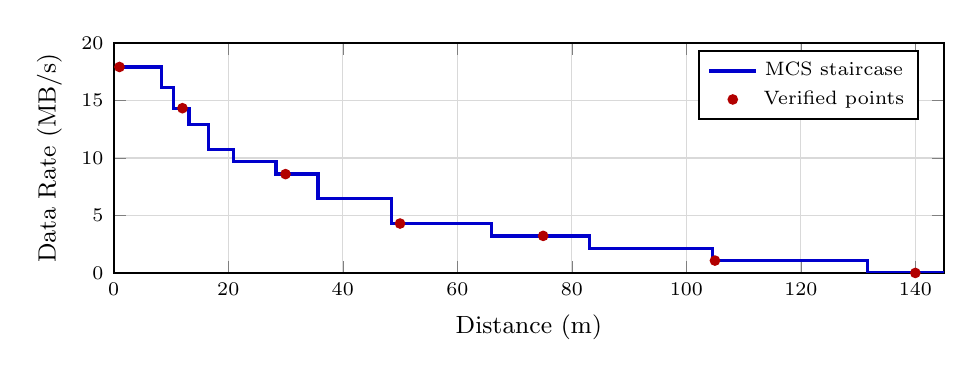
\begin{tikzpicture}
\begin{axis}[
  width=\columnwidth,
  height=4.5cm,
  xlabel={Distance (m)},
  ylabel={Data Rate (MB/s)},
  xmin=0, xmax=145,
  ymin=0, ymax=20,
  grid=major,
  grid style={gray!30},
  thick,
  legend pos=north east,
  legend style={font=\scriptsize},
  every axis label/.style={font=\small},
  tick label style={font=\scriptsize},
]
\addplot[blue!80!black, very thick]
  coordinates {
    (1, 17.925) (8.30, 17.925)
    (8.30, 16.125) (10.46, 16.125)
    (10.46, 14.338) (13.16, 14.338)
    (13.16, 12.900) (16.57, 12.900)
    (16.57, 10.750) (20.86, 10.750)
    (20.86, 9.675) (28.36, 9.675)
    (28.36, 8.600) (35.70, 8.600)
    (35.70, 6.450) (48.53, 6.450)
    (48.53, 4.300) (65.97, 4.300)
    (65.97, 3.225) (83.05, 3.225)
    (83.05, 2.150) (104.55, 2.150)
    (104.55, 1.075) (131.62, 1.075)
    (131.62, 0) (145, 0)
  };
\addplot[only marks, mark=*, mark size=1.5pt, red!70!black]
  coordinates {
    (1, 17.925) (12, 14.338) (30, 8.600) (50, 4.300)
    (75, 3.225) (105, 1.075) (140, 0)
  };
\legend{MCS staircase, Verified points}
\end{axis}
\end{tikzpicture}
\caption{Experiment 1: PHY data rate vs.\ link distance showing discrete MCS
  transitions (802.11ax, 5\,GHz, $n{=}3$).  Red dots mark experimentally
  verified data points from \Cref{tab:exp1}.}
\label{fig:exp1}
\end{figure}

\subsubsection{Experiment 2: Parallel Link Separation}

Two parallel 30\,m links separated vertically by distances from 5\,m to
200\,m.  \Cref{fig:exp2} illustrates the three interference regimes.
At separation $\leq 70$\,m, all node pairs are within the carrier
sensing range (71.2\,m), so the links \emph{contend} via Bianchi's model:
each gets $\eta(2)/2 \approx 0.44$ of the base rate 8.6\,MB/s $= 3.79$\,MB/s.
At separation $\geq 75$\,m, the links become hidden terminals, and SINR
degradation determines the effective rate.

Notably, the effective rate \emph{drops} at the CS range boundary---from
3.79\,MB/s (contention) to 3.23\,MB/s (hidden terminal at 75\,m)---before
recovering at larger separations.  This non-monotonic behavior is the
classic \emph{hidden terminal effect}: within sensing range, links coordinate
via CSMA/CA and time-share the channel fairly (each receiving 44\% of the
full 8.6\,MB/s); just outside sensing range, links transmit simultaneously
without coordination, and the resulting mutual interference degrades each
receiver's SINR enough to force a lower MCS rate (from MCS~5 to MCS~2).
The hidden terminal regime is thus \emph{worse} than fair contention sharing
at close range.  As separation increases further, interference power
diminishes: SINR recovers to MCS~3 (4.3\,MB/s) at 90\,m and MCS~4
(6.45\,MB/s) at 130\,m.  All 15 data points match predictions exactly.

\begin{figure}[t]
\centering
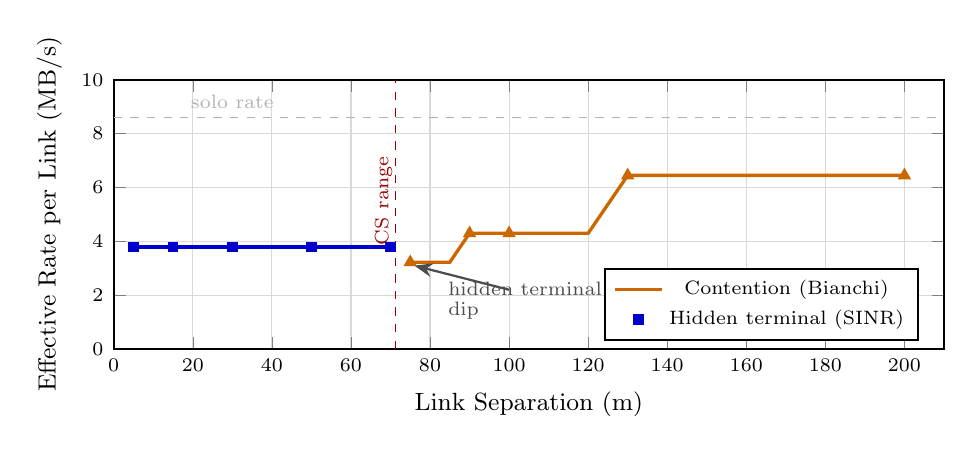
\begin{tikzpicture}
\begin{axis}[
  width=\columnwidth,
  height=5cm,
  xlabel={Link Separation (m)},
  ylabel={Effective Rate per Link (MB/s)},
  xmin=0, xmax=210,
  ymin=0, ymax=10,
  grid=major,
  grid style={gray!30},
  thick,
  every axis label/.style={font=\small},
  tick label style={font=\scriptsize},
  legend pos=south east,
  legend style={font=\scriptsize},
]
% Solo rate reference
\addplot[dashed, gray!60, thin] coordinates {(0, 8.600) (210, 8.600)};
\node[font=\scriptsize, gray!60] at (axis cs:30,9.2) {solo rate};

% CS range marker
\draw[dashed, red!60!black, thin] (axis cs:71.2,0) -- (axis cs:71.2,10);
\node[font=\scriptsize, red!60!black, rotate=90, anchor=south] at (axis cs:73,5.5) {CS range};

% Contention regime
\addplot[blue!80!black, very thick]
  coordinates {
    (5, 3.787) (10, 3.787) (15, 3.787) (20, 3.787) (25, 3.787)
    (30, 3.787) (35, 3.787) (40, 3.787) (45, 3.787) (50, 3.787)
    (55, 3.787) (60, 3.787) (65, 3.787) (70, 3.787)
  };

% Hidden terminal regime
\addplot[orange!80!black, very thick]
  coordinates {
    (75, 3.225) (80, 3.225) (85, 3.225)
    (90, 4.300) (95, 4.300) (100, 4.300) (110, 4.300) (120, 4.300)
    (130, 6.450) (140, 6.450) (150, 6.450) (175, 6.450) (200, 6.450)
  };

\addplot[only marks, mark=square*, mark size=1.5pt, blue!80!black]
  coordinates {
    (5, 3.787) (15, 3.787) (30, 3.787) (50, 3.787) (70, 3.787)
  };
\addplot[only marks, mark=triangle*, mark size=2pt, orange!80!black]
  coordinates {
    (75, 3.225) (90, 4.300) (100, 4.300) (130, 6.450) (200, 6.450)
  };

% Annotation: hidden terminal dip
\draw[-{Stealth}, thick, black!70] (axis cs:100,2.2) -- (axis cs:76,3.1);
\node[font=\scriptsize, anchor=west, align=left, black!70] at (axis cs:82,1.8)
  {hidden terminal\\[-1pt]dip};

\legend{, , Contention (Bianchi), Hidden terminal (SINR), , }
\end{axis}
\end{tikzpicture}
\caption{Experiment 2: Effective per-link rate vs.\ separation for two
  parallel 30\,m links.  Below the CS range (71.2\,m), links contend via
  Bianchi's model.  Above it, hidden terminal SINR degradation causes a
  non-monotonic \emph{dip}: the rate drops from 3.79 to 3.23\,MB/s at the
  boundary because uncoordinated simultaneous transmissions degrade SINR
  more than fair time-sharing reduces throughput.  Rate recovers as
  interference power falls with increasing distance.}
\label{fig:exp2}
\end{figure}

\subsubsection{Experiment 7: N-Way Bianchi Contention Scaling}

\Cref{tab:exp7} shows per-link throughput as the number of contending
30\,m links (at 5\,m separation) increases from $n{=}2$ to $n{=}8$.
Bianchi MAC efficiency $\eta(n)$ decreases from 0.881 to 0.726; the
per-station share $\eta(n)/n$ falls correspondingly.  All seven data
points match analytical predictions exactly.

\begin{table}[t]
\centering
\caption{Experiment 7: N-way Bianchi contention scaling (30\,m links at 5\,m
separation).  $\eta(n)$ is the Bianchi MAC efficiency.}
\label{tab:exp7}
\begin{tabular}{@{}rrrrrr@{}}
\toprule
$n$ & $\eta(n)$ & $\eta(n)/n$ & \textbf{Pred(MB/s)} & \textbf{Sim(MB/s)} \\
\midrule
2 & 0.881 & 0.440 & 3.787 & 3.787 \\
3 & 0.859 & 0.286 & 2.461 & 2.461 \\
4 & 0.837 & 0.209 & 1.799 & 1.799 \\
5 & 0.818 & 0.164 & 1.407 & 1.407 \\
6 & 0.802 & 0.134 & 1.149 & 1.149 \\
7 & 0.788 & 0.113 & 0.968 & 0.968 \\
8 & 0.726 & 0.091 & 0.780 & 0.780 \\
\bottomrule
\end{tabular}
\end{table}

\subsubsection{Additional Validation Experiments}

Six additional experiments validate: (4)~three-link topologies with mixed
contention and hidden terminal regimes, (5)~staggered transfer starts with
dynamic recalculation, (6)~per-link bandwidth sharing with multiple flows,
(8)~five-link hidden terminal cascades with different data sizes, and
(9)~combined bandwidth sharing with hidden terminal interference.  All pass.


\subsection{External Validation Against Bianchi (2000)}
\label{sec:external_val}

Internal validation confirms self-consistency but does not establish
that our implementation of Bianchi's equations is correct.  We therefore
reproduce the numerical results from Bianchi's original paper
\cite{bianchi2000} using his exact parameters: FHSS 1\,Mbps basic
access (no RTS/CTS), with slot duration 50\,$\mu$s, SIFS 28\,$\mu$s,
DIFS 128\,$\mu$s, propagation delay 1\,$\mu$s, payload 8184 bits,
MAC header 272 bits, PHY header 128 bits, and ACK 112 bits.

\subsubsection{Table III Reproduction}

\Cref{tab:bianchi_table3} compares our computed normalized saturation
throughput $S$ against the values published in Bianchi's Table~III for
$W{=}32$, $m{=}3$.  At $n{=}2$, our solver computes $S = 0.847311$
versus the published $0.8473$ (relative error $0.001\%$).  At $n{=}3$,
we compute $S = 0.836828$ versus $0.8368$ (relative error $0.003\%$).
These sub-basis-point differences are consistent with rounding in the
published table.

\begin{table}[t]
\centering
\caption{Reproduction of Bianchi~\cite{bianchi2000} Table~III:
normalized saturation throughput $S$ for $W{=}32$, $m{=}3$.}
\label{tab:bianchi_table3}
\begin{tabular}{@{}rrrr@{}}
\toprule
$n$ & \textbf{Computed} & \textbf{Published} & \textbf{Rel.\ Error} \\
\midrule
2  & 0.847311 & 0.8473 & 0.001\% \\
3  & 0.836828 & 0.8368 & 0.003\% \\
\bottomrule
\end{tabular}
\end{table}

Our solver for the coupled equations (\Cref{eq:tau,eq:p}) uses a bisection
method rather than simple fixed-point iteration.  Simple iteration can
oscillate when the contention window is small or the number of stations is
large, because the mapping can have a slope exceeding unity near the fixed
point.  Bisection is guaranteed to converge within
$\lceil \log_2(1/\epsilon) \rceil$ iterations for any tolerance $\epsilon$.
We use $\epsilon = 10^{-12}$, requiring at most 40 bisection steps.

\subsubsection{Figure 6 Reproduction}

We also reproduce Bianchi's Figure~6 throughput curves for two
configurations: $W{=}32$, $m{=}5$ (CW$_{\max}{=}1024$) and $W{=}128$,
$m{=}3$ (CW$_{\max}{=}1024$).  \Cref{fig:bianchi_fig6} plots the
computed normalized throughput $S$ across the full range of station
counts from $n{=}5$ to $n{=}50$.  \Cref{tab:bianchi_fig6} presents
the numerical values underlying these curves.

Several features of these curves merit discussion.  First, both
configurations exhibit the expected monotonic decrease in throughput with
increasing $n$: as more stations contend, collision overhead grows and
the fraction of time spent on successful transmissions decreases.
Second, the $W{=}128$ curve shows a slight non-monotonicity between
$n{=}5$ ($S = 0.825$) and $n{=}10$ ($S = 0.826$).  This occurs because
the larger initial contention window is oversized for a small number of
stations, causing excessive idle time; as $n$ increases from 5 to 10,
the window becomes better matched to the contention level before
collision losses begin to dominate.  This non-monotonicity is consistent
with Bianchi's published results and would not be captured by simpler
throughput models.  Third, the gap between the two curves narrows at
large $n$: at $n{=}50$, $W{=}128$ achieves $S = 0.725$ versus $S = 0.611$
for $W{=}32$ (a 19\% advantage), whereas at $n{=}5$ the gap is only 2\%.
This confirms the well-known principle that larger contention windows
provide greater benefit in high-contention regimes.

\begin{table}[t]
\centering
\caption{Numerical values for Bianchi Figure~6 reproduction:
normalized saturation throughput $S$ for two $(W, m)$ configurations.}
\label{tab:bianchi_fig6}
\begin{tabular}{@{}rrr@{}}
\toprule
$n$ & $S$ ($W{=}32, m{=}5$) & $S$ ($W{=}128, m{=}3$) \\
\midrule
5  & 0.8102 & 0.8250 \\
10 & 0.7579 & 0.8263 \\
15 & 0.7231 & 0.8130 \\
20 & 0.6975 & 0.7981 \\
25 & 0.6772 & 0.7837 \\
30 & 0.6603 & 0.7702 \\
35 & 0.6457 & 0.7577 \\
40 & 0.6329 & 0.7461 \\
45 & 0.6214 & 0.7353 \\
50 & 0.6109 & 0.7252 \\
\bottomrule
\end{tabular}
\end{table}

\begin{figure}[t]
\centering
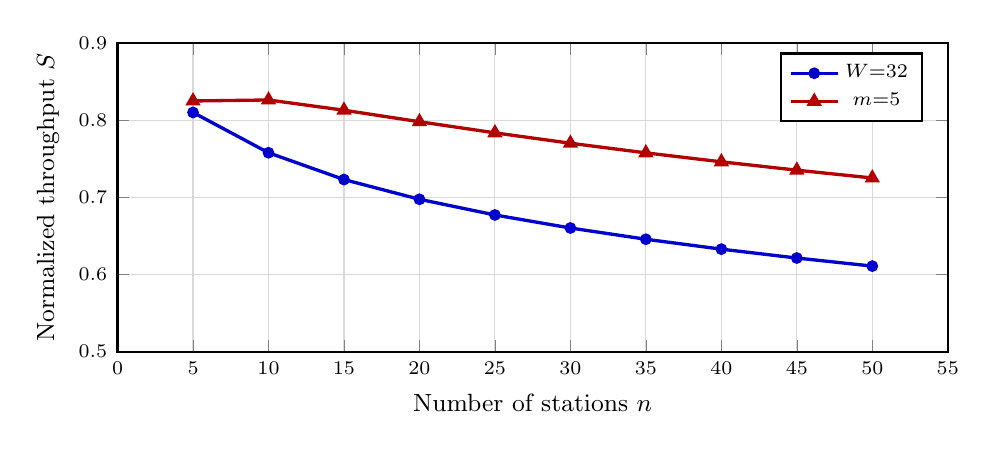
\begin{tikzpicture}
\begin{axis}[
  width=\columnwidth,
  height=5.5cm,
  xlabel={Number of stations $n$},
  ylabel={Normalized throughput $S$},
  xmin=0, xmax=55,
  ymin=0.5, ymax=0.9,
  grid=major,
  grid style={gray!30},
  thick,
  every axis label/.style={font=\small},
  tick label style={font=\scriptsize},
  legend pos=north east,
  legend style={font=\scriptsize},
]
% W=32, m=5
\addplot[blue!80!black, very thick, mark=*, mark size=1.5pt]
  coordinates {
    (5, 0.810153) (10, 0.75788) (15, 0.723136) (20, 0.697548)
    (25, 0.677235) (30, 0.660309) (35, 0.645739) (40, 0.632901)
    (45, 0.621392) (50, 0.610936)
  };
% W=128, m=3
\addplot[red!70!black, very thick, mark=triangle*, mark size=2pt]
  coordinates {
    (5, 0.825024) (10, 0.826309) (15, 0.813031) (20, 0.798105)
    (25, 0.783692) (30, 0.770226) (35, 0.757731) (40, 0.746123)
    (45, 0.7353) (50, 0.725166)
  };
\legend{$W{=}32$, $m{=}5$, $W{=}128$, $m{=}3$}
\end{axis}
\end{tikzpicture}
\caption{Reproduction of Bianchi~\cite{bianchi2000} Figure~6:
  normalized saturation throughput vs.\ number of stations for two
  $(W, m)$ configurations.  Computed using Bianchi's exact FHSS
  parameters (1\,Mbps basic access, no RTS/CTS).  The $W{=}128$
  curve's slight non-monotonicity between $n{=}5$ and $n{=}10$ is
  consistent with Bianchi's published results.}
\label{fig:bianchi_fig6}
\end{figure}


%% ============================================================
\section{Experimental Evaluation}
\label{sec:eval}

Having validated the correctness of \ncsim{}'s WiFi model, we now turn to
the central question that motivates this work: does ignoring wireless
interference merely produce inaccurate makespan estimates, or does it lead
to fundamentally wrong conclusions about which scheduling and routing
policies are superior?  We evaluate \ncsim{} through four sets of
experiments that progressively build the case.  First, we compare routing
strategies to demonstrate that the choice of routing algorithm interacts
non-trivially with interference.  Second, we quantify the magnitude of
interference impact on makespan predictions.  Third, we execute a full
108-run factorial comparison revealing that interference changes \emph{which
scheduler wins} in nearly 40\% of scenarios.  Finally, sensitivity
analyses identify the parameter regimes where interference is most
consequential.

All experiments use 802.11ax at 5\,GHz with a path loss exponent of
$n = 3$ (except where explicitly varied), heterogeneous compute capacities
(80--300 units/s), 10\,MB data payloads per DAG edge, and deterministic
seed~42.

\subsection{Routing Strategy Comparison}
\label{sec:routing_eval}

We compare widest-path and shortest-path routing under HEFT scheduling with
the \texttt{csma\_bianchi} interference model across grid mesh networks of
three sizes (2$\times$2, 3$\times$3, 4$\times$4) and three DAG complexities
(5, 10, and 20 tasks).  All links are wireless with 40\,m grid spacing.
Nodes have heterogeneous compute capacities (80--300 units/s).
\Cref{tab:routing} shows the results.

\Cref{fig:routing_diamond} illustrates \emph{why} routing strategy matters
using a diamond topology with asymmetric paths.  The widest-path algorithm
selects the high-bandwidth bottom path (200\,MB/s, 0.1\,s latency per hop),
achieving a makespan of 2.6\,s.  Shortest-path selects the low-latency top
path (20\,MB/s, 0.001\,s per hop), yielding 7.0\,s---a 2.7$\times$ slowdown
because the 100\,MB transfer dominates the total time.

\begin{figure}[t]
\centering
\begin{subfigure}[b]{\columnwidth}
\centering
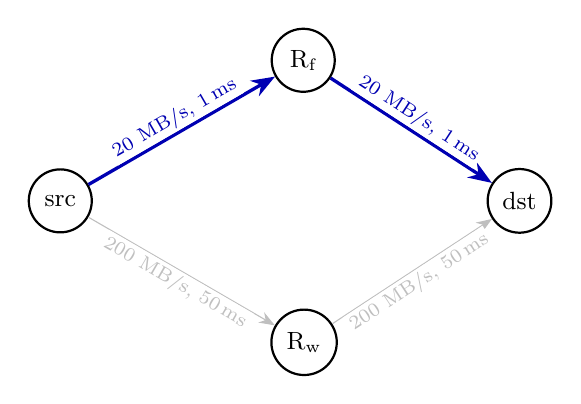
\begin{tikzpicture}[
  node distance=2cm and 2.8cm,
  nnode/.style={circle, draw, thick, minimum size=8mm, font=\small},
  sel/.style={-{Stealth[length=3mm]}, very thick, blue!70!black},
  dim/.style={-{Stealth[length=2mm]}, thin, gray!50},
  lbl/.style={font=\scriptsize, fill=white, inner sep=1pt},
]
  \node[nnode] (src) {src};
  \node[nnode, above right=1.2cm and 2.5cm of src] (fast) {R\textsubscript{f}};
  \node[nnode, below right=1.2cm and 2.5cm of src] (wide) {R\textsubscript{w}};
  \node[nnode, right=5cm of src] (dst) {dst};

  % Shortest path highlighted
  \draw[sel] (src) -- node[lbl, above, sloped] {20 MB/s, 1\,ms} (fast);
  \draw[sel] (fast) -- node[lbl, above, sloped] {20 MB/s, 1\,ms} (dst);

  % Wide path dimmed
  \draw[dim] (src) -- node[lbl, below, sloped] {200 MB/s, 50\,ms} (wide);
  \draw[dim] (wide) -- node[lbl, below, sloped] {200 MB/s, 50\,ms} (dst);
\end{tikzpicture}
\caption{Shortest-path routing selects the top path (lower latency).\\
  Makespan: $1.0 + (100/20 + 0.002) + 1.0 = 7.0$\,s.}
\end{subfigure}

\vspace{6pt}

\begin{subfigure}[b]{\columnwidth}
\centering
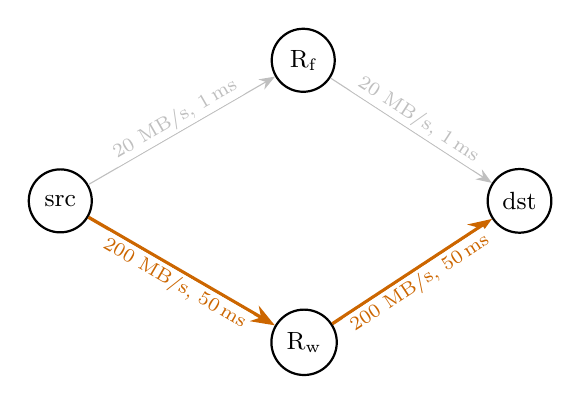
\begin{tikzpicture}[
  node distance=2cm and 2.8cm,
  nnode/.style={circle, draw, thick, minimum size=8mm, font=\small},
  sel/.style={-{Stealth[length=3mm]}, very thick, orange!80!black},
  dim/.style={-{Stealth[length=2mm]}, thin, gray!50},
  lbl/.style={font=\scriptsize, fill=white, inner sep=1pt},
]
  \node[nnode] (src) {src};
  \node[nnode, above right=1.2cm and 2.5cm of src] (fast) {R\textsubscript{f}};
  \node[nnode, below right=1.2cm and 2.5cm of src] (wide) {R\textsubscript{w}};
  \node[nnode, right=5cm of src] (dst) {dst};

  % Fast path dimmed
  \draw[dim] (src) -- node[lbl, above, sloped] {20 MB/s, 1\,ms} (fast);
  \draw[dim] (fast) -- node[lbl, above, sloped] {20 MB/s, 1\,ms} (dst);

  % Widest path highlighted
  \draw[sel] (src) -- node[lbl, below, sloped] {200 MB/s, 50\,ms} (wide);
  \draw[sel] (wide) -- node[lbl, below, sloped] {200 MB/s, 50\,ms} (dst);
\end{tikzpicture}
\caption{Widest-path routing selects the bottom path (higher bandwidth).\\
  Makespan: $1.0 + (100/200 + 0.1) + 1.0 = 2.6$\,s.}
\end{subfigure}
\caption{Routing strategy comparison on a diamond topology with a 100\,MB
  transfer.  When transfer size dominates, widest-path outperforms
  shortest-path by 2.7$\times$.}
\label{fig:routing_diamond}
\end{figure}

\begin{table}[t]
\centering
\caption{Routing comparison: makespan (seconds) for widest-path (W) vs.\
shortest-path (S) under HEFT with \texttt{csma\_bianchi}.}
\label{tab:routing}
\begin{tabular}{@{}llrrr@{}}
\toprule
\textbf{Network} & \textbf{DAG} & \textbf{W (s)} & \textbf{S (s)} & \textbf{Winner} \\
\midrule
\multirow{3}{*}{2$\times$2 (4 nodes)}
  & 5 tasks   & 11.43  & 11.43  & Tie \\
  & 10 tasks  & 20.52  & 26.03  & Widest \\
  & 20 tasks  & 51.65  & 38.94  & Shortest \\
\midrule
\multirow{3}{*}{3$\times$3 (9 nodes)}
  & 5 tasks   & 12.37  & 12.37  & Tie \\
  & 10 tasks  & 29.52  & 25.04  & Shortest \\
  & 20 tasks  & 46.01  & 40.82  & Shortest \\
\midrule
\multirow{3}{*}{4$\times$4 (16 nodes)}
  & 5 tasks   & 315.20 & 8.93   & Shortest \\
  & 10 tasks  & 967.21 & 434.13 & Shortest \\
  & 20 tasks  & 1472.3 & 671.65 & Shortest \\
\bottomrule
\end{tabular}
\end{table}

\textbf{Key findings.}
Shortest-path routing wins in 6 of 9 configurations with 2 ties.  The
advantage is most pronounced in the 4$\times$4 grid, where widest-path
routing selects longer paths with higher bottleneck bandwidth but incurs
substantially more wireless interference due to multi-hop transmissions
traversing more contention domains.  In the 4$\times$4 grid with 5 tasks,
widest-path achieves a makespan of 315.2\,s compared to 8.9\,s for
shortest-path---a $35\times$ difference---because the widest paths route
transfers through 3--4 hops across the full grid diameter, creating
overlapping contention domains that reduce effective bandwidth to a
fraction of the solo rate.

However, widest-path routing does win in the 2$\times$2 grid with 10 tasks,
achieving 20.5\,s versus 26.0\,s for shortest-path.  In this small
topology, contention is manageable (at most 12 links in the conflict graph)
and the higher bottleneck bandwidth of widest paths outweighs the modest
interference penalty.  This demonstrates that routing strategy choice is
both topology- and workload-dependent: what is optimal in a small, lightly
contended network can be catastrophically wrong in a larger, denser one.
Such topology-dependent reversals underscore the value of simulating the
full compute-network interaction rather than selecting routing strategies
based on bandwidth alone.


\subsection{Interference Impact Analysis}
\label{sec:interference_eval}

We measure the impact of CSMA/CA interference by running each of the nine
grid-network scenarios with the \texttt{csma\_bianchi} model versus no
interference (\texttt{none}), both using shortest-path routing and HEFT.
To ensure a fair comparison, WiFi-derived PHY rates are used as explicit
link bandwidths in both modes so that the only difference is the presence
or absence of contention and hidden terminal effects.
\Cref{tab:interference} summarizes the results.

\begin{table}[t]
\centering
\caption{Interference impact: makespan (seconds) without interference vs.\
with \texttt{csma\_bianchi}, using shortest-path routing and HEFT scheduling.}
\label{tab:interference}
\begin{tabular}{@{}llrrr@{}}
\toprule
\textbf{Network} & \textbf{DAG} & \textbf{None (s)} & \textbf{Bianchi (s)} & \textbf{Slowdown} \\
\midrule
\multirow{3}{*}{2$\times$2 (4n, 12 links)}
  & 5 tasks   & 11.43  & 11.43  & 0\%     \\
  & 10 tasks  & 18.10  & 26.03  & +44\%   \\
  & 20 tasks  & 25.60  & 39.98  & +56\%   \\
\midrule
\multirow{3}{*}{3$\times$3 (9n, 32 links)}
  & 5 tasks   & 8.43   & 12.37  & +47\%   \\
  & 10 tasks  & 11.99  & 25.04  & +109\%  \\
  & 20 tasks  & 19.03  & 52.07  & +174\%  \\
\midrule
\multirow{3}{*}{4$\times$4 (16n, 68 links)}
  & 5 tasks   & 8.93   & 8.93   & 0\%     \\
  & 10 tasks  & 14.96  & 436.95 & +2821\% \\
  & 20 tasks  & 15.87  & 225.67 & +1322\% \\
\bottomrule
\end{tabular}
\end{table}

\textbf{Key findings.}
Interference impact ranges from 0\% (when few concurrent transfers avoid
contention) to over 2800\% in the 4$\times$4 grid with 10 tasks.  Several
patterns emerge:

\begin{itemize}[itemsep=1pt,leftmargin=*]
\item \textbf{Small DAGs escape contention.}  With only 5 tasks, the
  2$\times$2 and 4$\times$4 grids show zero slowdown because HEFT spreads
  tasks sufficiently that transfers rarely overlap.
\item \textbf{Denser networks amplify interference.}  The 3$\times$3 grid
  (32 links) shows 47--174\% slowdown, while the 4$\times$4 grid (68 links)
  shows up to 2821\%.  More links create larger conflict neighborhoods.
\item \textbf{Dense interference creates cascading delays.}  In the
  4$\times$4 grid, HEFT distributes tasks across 16 nodes assuming
  uncontested bandwidth.  During execution, many simultaneous transfers
  contend, reducing effective rates and causing HEFT's schedule to
  become severely suboptimal.
\end{itemize}

\noindent These results demonstrate that ignoring wireless interference in
scheduling can lead to order-of-magnitude performance prediction errors,
motivating the physically-grounded model in \ncsim{}.


\subsection{Scheduler Comparison and Rank Inversions}
\label{sec:scheduler_eval}

The interference impact results above suggest a deeper question: does
ignoring interference merely produce inaccurate makespan predictions, or
does it lead to wrong \emph{choices} among schedulers?  To answer this, we
execute a full factorial comparison: 3 networks $\times$ 3 DAGs $\times$
3 schedulers (HEFT, CPOP, RoundRobin) $\times$ 2 routings $\times$ 2
interference models $= 108$ simulation runs.  All runs use 802.11ax at
5\,GHz, heterogeneous compute capacities, and seed~42.

For each of the 18 (network, DAG, routing) triples, we identify the best
scheduler under each interference model.  A \emph{rank inversion} occurs
when the winning scheduler changes between the interference-free and
interference-aware models.  The \emph{scheduling regret} is the relative
performance penalty from deploying the interference-free-optimal scheduler
in the presence of interference.

\Cref{tab:winner_matrix} presents the results.  The key statistics are:
\begin{itemize}[itemsep=1pt,leftmargin=*]
\item \textbf{Rank inversion rate: 38.9\%} (7 of 18 triples).
\item \textbf{Mean relative regret: 66.0\%} across all 18 triples.
\item \textbf{Maximum relative regret: 484.1\%} ($4\times4$ grid,
  5-task DAG, widest\_path: HEFT chosen under ``none'' gives
  315.2\,s, but round\_robin achieves 54.0\,s under csma\_bianchi).
\end{itemize}

\begin{table*}[t]
\centering
\caption{Winning scheduler per (network, DAG, routing) triple under
  interference-free (``None'') and csma\_bianchi (``Bian.'') models.
  Bold entries indicate rank inversions.  Makespan in seconds shown
  in parentheses.}
\label{tab:winner_matrix}
\begin{tabular}{@{}ll|ll|ll@{}}
\toprule
& & \multicolumn{2}{c|}{\textbf{Widest-path}} &
  \multicolumn{2}{c}{\textbf{Shortest-path}} \\
\textbf{Network} & \textbf{DAG} &
  \textbf{None} & \textbf{Bian.} &
  \textbf{None} & \textbf{Bian.} \\
\midrule
\multirow{3}{*}{$2\times2$}
  & 5 tasks  & HEFT (11.4)  & HEFT (11.4)   & HEFT (11.4) & HEFT (11.4) \\
  & 10 tasks & HEFT (18.1)  & HEFT (20.1)   & HEFT (18.1) & HEFT (26.0) \\
  & 20 tasks & CPOP (26.2)  & CPOP (43.9)   & HEFT (27.8) & HEFT (36.5) \\
\midrule
\multirow{3}{*}{$3\times3$}
  & 5 tasks  & HEFT (8.4)   & HEFT (12.4)   & HEFT (8.4) & HEFT (12.4) \\
  & 10 tasks & HEFT (13.3)  & \textbf{CPOP (36.3)} & CPOP (13.7) & \textbf{HEFT (25.0)} \\
  & 20 tasks & CPOP (16.3)  & CPOP (69.3)   & CPOP (20.0) & \textbf{HEFT (55.3)} \\
\midrule
\multirow{3}{*}{$4\times4$}
  & 5 tasks  & HEFT (8.2)   & \textbf{RR (54.0)}  & HEFT (8.9) & HEFT (8.9) \\
  & 10 tasks & HEFT (16.4)  & \textbf{RR (253.9)} & HEFT (15.0) & \textbf{RR (184.8)} \\
  & 20 tasks & HEFT (22.2)  & \textbf{RR (937.4)} & HEFT (15.9) & HEFT (676.2) \\
\bottomrule
\end{tabular}
\end{table*}

\textbf{HEFT dominates under interference-free models.}  Under the
``none'' interference model, HEFT or CPOP wins in all 18 triples.  This
is expected: both algorithms optimize the critical path by distributing
tasks across nodes to maximize parallelism, assuming uncontested bandwidth.
The sophisticated scheduling logic of HEFT and CPOP provides clear
advantages when the network behaves as these algorithms assume it will.

\textbf{Round-robin wins in large networks under interference.}
In the $4\times4$ grid with csma\_bianchi and widest-path routing,
round-robin wins for all three DAG sizes---a striking reversal.  The
mechanism is clear: HEFT spreads tasks across many of the 16 available
nodes to exploit parallelism, but this creates many concurrent multi-hop
transfers that contend on shared wireless channels.  Round-robin's simpler
placement cycles through nodes in order, which tends to concentrate work
on nearby nodes with fewer concurrent transfers and thus less contention.

To illustrate this mechanism concretely, consider the most dramatic rank
inversion: the $4\times4$ grid with 10 tasks and widest-path routing.
Under the interference-free model, HEFT achieves a makespan of 16.4\,s by
distributing tasks across 10 of the 16 nodes, creating up to 8 concurrent
inter-node transfers that exploit the assumed 6.45--8.6\,MB/s link
bandwidths.  However, under csma\_bianchi, these 8 concurrent transfers
contend on overlapping conflict graph neighborhoods: each transfer's
effective bandwidth drops to a fraction of its solo rate as the Bianchi
model allocates channel time among contenders.  The resulting makespan
\emph{explodes} to 1,396.9\,s---an 85$\times$ blowup.  In contrast,
round-robin achieves 253.9\,s under the same interference model.
Although round-robin makes no attempt to optimize the critical path, its
placement pattern generates fewer concurrent transfers, resulting in less
severe contention.  The scheduling regret---the penalty for choosing HEFT
based on the interference-free evaluation---is 450\%.  A researcher
evaluating these schedulers without interference modeling would confidently
select HEFT, unaware that it produces $5.5\times$ worse performance than
the ``naive'' round-robin baseline.

\textbf{Routing modulates the effect.}  Shortest-path routing mitigates
rank inversions in some cases by reducing the number of hops per transfer
and thus the number of contention domains traversed.  The $4\times4$ /
5-task scenario shows a rank inversion under widest-path routing (484\%
regret) but not under shortest-path (zero regret).  However, shortest-path
does not eliminate inversions entirely: in the $4\times4$ / 10-task
scenario, the inversion persists even with shortest-path routing (135\%
regret), because the DAG is large enough to generate concurrent transfers
even along short paths.

\Cref{fig:regret_scatter} visualizes the regret: for each triple, an arrow
connects the oracle makespan (best scheduler under csma\_bianchi) to the
naive makespan (scheduler chosen under ``none,'' run under csma\_bianchi).
The most dramatic cases occur in the $4\times4$ grid where HEFT's
parallelism-maximizing placement creates dense contention.

\begin{figure}[t]
\centering
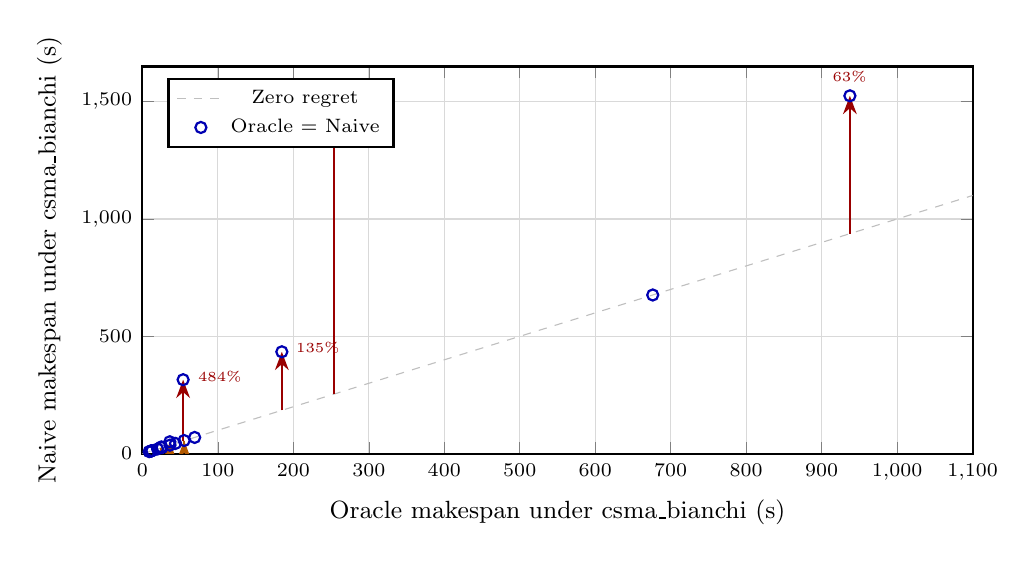
\begin{tikzpicture}
\begin{axis}[
  width=\columnwidth,
  height=6.5cm,
  xlabel={Oracle makespan under csma\_bianchi (s)},
  ylabel={Naive makespan under csma\_bianchi (s)},
  xmin=0, xmax=1100,
  ymin=0, ymax=1650,
  grid=major,
  grid style={gray!30},
  thick,
  every axis label/.style={font=\small},
  tick label style={font=\scriptsize},
  legend pos=north west,
  legend style={font=\scriptsize},
]
% Diagonal (zero regret line)
\addplot[dashed, gray!50, thin, domain=0:1100] {x};

% Oracle points
\addplot[only marks, mark=o, mark size=2pt, blue!70!black]
  coordinates {
    (11.434, 11.434) (11.434, 11.434)
    (20.071, 20.071) (26.032, 26.032)
    (43.887, 43.887) (36.510, 36.510)
    (12.375, 12.375) (12.375, 12.375)
    (36.325, 50.819) (25.040, 28.832)
    (69.282, 69.282) (55.312, 56.102)
    (53.967, 315.197) (8.934, 8.934)
    (253.907, 1396.857) (184.773, 434.129)
    (937.411, 1524.713) (676.194, 676.194)
  };

% Regret arrows for inversions
\draw[-{Stealth}, red!60!black, thick]
  (axis cs:53.967, 53.967) -- (axis cs:53.967, 315.197);
\draw[-{Stealth}, red!60!black, thick]
  (axis cs:253.907, 253.907) -- (axis cs:253.907, 1396.857);
\draw[-{Stealth}, red!60!black, thick]
  (axis cs:184.773, 184.773) -- (axis cs:184.773, 434.129);
\draw[-{Stealth}, red!60!black, thick]
  (axis cs:937.411, 937.411) -- (axis cs:937.411, 1524.713);
\draw[-{Stealth}, orange!70!black]
  (axis cs:36.325, 36.325) -- (axis cs:36.325, 50.819);
\draw[-{Stealth}, orange!70!black]
  (axis cs:25.040, 25.040) -- (axis cs:25.040, 28.832);
\draw[-{Stealth}, orange!70!black]
  (axis cs:55.312, 55.312) -- (axis cs:55.312, 56.102);

% Labels for extreme points
\node[font=\tiny, anchor=west, red!60!black] at (axis cs:60, 330)
  {484\%};
\node[font=\tiny, anchor=west, red!60!black] at (axis cs:260, 1410)
  {450\%};
\node[font=\tiny, anchor=west, red!60!black] at (axis cs:190, 450)
  {135\%};
\node[font=\tiny, anchor=south, red!60!black] at (axis cs:937, 1540)
  {63\%};

\legend{Zero regret, Oracle $=$ Naive}
\end{axis}
\end{tikzpicture}
\caption{Makespan regret scatter plot.  Each arrow connects the oracle
  makespan (best scheduler under csma\_bianchi) to the naive makespan
  (scheduler chosen under interference-free model, run under
  csma\_bianchi).  Red arrows indicate rank inversions; orange arrows
  indicate moderate regret.  7 of 18 triples exhibit rank inversions.}
\label{fig:regret_scatter}
\end{figure}

These results demonstrate a key capability of \ncsim{}: by jointly modeling
scheduling and wireless interference, it reveals that interference-free
evaluations can lead not merely to inaccurate estimates but to
systematically wrong policy choices---a finding that would be invisible to
tools that abstract away wireless contention.


\subsection{Sensitivity Analysis}
\label{sec:sensitivity}

The results above demonstrate that wireless interference can dramatically
affect scheduler rankings.  However, a natural question arises: under what
conditions is interference most consequential, and when can it safely be
ignored?  To address this question, we conduct three sensitivity sweeps
that vary the key parameters affecting interference severity: the RF
propagation environment (path loss exponent), the communication-to-computation
ratio (data size per DAG edge), and the level of concurrent workload
(number of simultaneous DAGs).

\subsubsection{Path Loss Exponent Sweep}

We sweep $n \in \{2.0, 2.5, 3.0, 3.5\}$ on the 3$\times$3 grid with the
10-task DAG, HEFT, and shortest-path routing.  (At $n{=}4.0$, 40\,m links
fall below the minimum MCS threshold and the network becomes disconnected.)

\Cref{fig:pathloss} reveals a dramatic regime transition.  At $n{=}2.0$
(near free-space propagation), the slowdown from interference is a modest
$1.33\times$: link rates are high (14.3\,MB/s for adjacent 40\,m links),
transfers complete quickly, and the time window during which links contend
is brief.  At $n{=}3.0$ (typical indoor or suburban), the slowdown doubles
to $2.0\times$ as link rates drop to 6.45\,MB/s and transfers take longer,
increasing the overlap between concurrent flows.  At $n{=}3.5$ (dense
indoor with many obstructions), the slowdown \emph{explodes} to
$104.6\times$.  The mechanism behind this cliff is a positive feedback
loop: lower link rates mean longer transfers, longer transfers mean more
temporal overlap, more overlap means more contention, and more contention
further reduces effective rates.  At $n{=}3.5$, adjacent links achieve only
3.2\,MB/s solo rate, and diagonal links drop to 1.1\,MB/s---barely above
the minimum MCS threshold.  Under contention, effective rates fall to
fractions of a MB/s, and transfers that would take seconds under
interference-free conditions instead take minutes.  At $n{=}4.0$, the
40\,m links fall below the minimum MCS threshold entirely and the network
becomes disconnected.

This regime transition has important practical implications.  For outdoor
deployments with clear line of sight ($n \approx 2.0$--$2.5$),
interference effects are moderate and may not change scheduler rankings.
However, for indoor or obstructed environments ($n \geq 3.0$), interference
modeling becomes essential.  The cliff between $n{=}3.0$ and $n{=}3.5$
is particularly notable because this range corresponds to common indoor
environments where many edge computing deployments operate.

\begin{figure}[t]
\centering
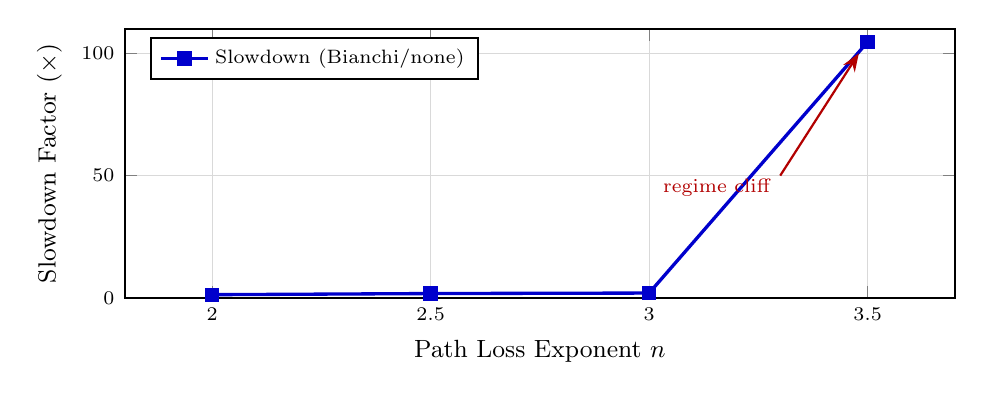
\begin{tikzpicture}
\begin{axis}[
  width=\columnwidth,
  height=5cm,
  xlabel={Path Loss Exponent $n$},
  ylabel={Slowdown Factor ($\times$)},
  xmin=1.8, xmax=3.7,
  ymin=0, ymax=110,
  grid=major,
  grid style={gray!30},
  thick,
  every axis label/.style={font=\small},
  tick label style={font=\scriptsize},
  legend pos=north west,
  legend style={font=\scriptsize},
  xtick={2.0, 2.5, 3.0, 3.5},
]
\addplot[blue!80!black, very thick, mark=square*, mark size=2pt]
  coordinates {
    (2.0, 1.33) (2.5, 1.80) (3.0, 2.00) (3.5, 104.61)
  };
\legend{Slowdown (Bianchi/none)}
\draw[-{Stealth}, thick, red!70!black] (axis cs:3.3,50) -- (axis cs:3.48,100);
\node[font=\scriptsize, red!70!black, anchor=east] at (axis cs:3.3,45) {regime cliff};
\end{axis}
\end{tikzpicture}
\caption{Interference slowdown vs.\ path loss exponent on 3$\times$3 grid
  (10-task DAG, HEFT, shortest-path).  A dramatic regime transition occurs
  between $n{=}3.0$ ($2\times$ slowdown) and $n{=}3.5$ ($105\times$).}
\label{fig:pathloss}
\end{figure}

\subsubsection{Communication-to-Computation Ratio}

The communication-to-computation ratio (CCR) determines the relative
importance of network transfer time versus compute time.  We sweep data
size per edge across $\{1, 2, 5, 10, 20, 50, 100\}$\,MB on the 3$\times$3
grid with HEFT and shortest-path routing, testing all three DAG types
(5, 10, and 20 tasks).  \Cref{fig:ccr} shows the interference slowdown
as a function of data size.

The results reveal a non-monotonic pattern: slowdown peaks at intermediate
CCR values (${\approx}0.3$--$1.1$) and decreases at both extremes.  The
mechanism differs at each end.  At low CCR (1--2\,MB), transfers complete
so quickly that the probability of temporal overlap between concurrent
flows is small, and contention has little opportunity to develop.  At very
high CCR (50--100\,MB), HEFT's scheduling logic recognizes the enormous
transfer costs and collapses tasks onto fewer nodes to avoid inter-node
communication entirely---a scheduling adaptation that eliminates contention
by eliminating transfers.  The interference ``danger zone'' lies in
between, where transfers are long enough to overlap but the scheduler
still distributes tasks across multiple nodes.  For the 20-task DAG, the
peak slowdown of $3.8\times$ occurs at 20\,MB per edge, corresponding to
a CCR of approximately 0.6 (where transfer time and compute time are
comparable).

\begin{figure}[t]
\centering
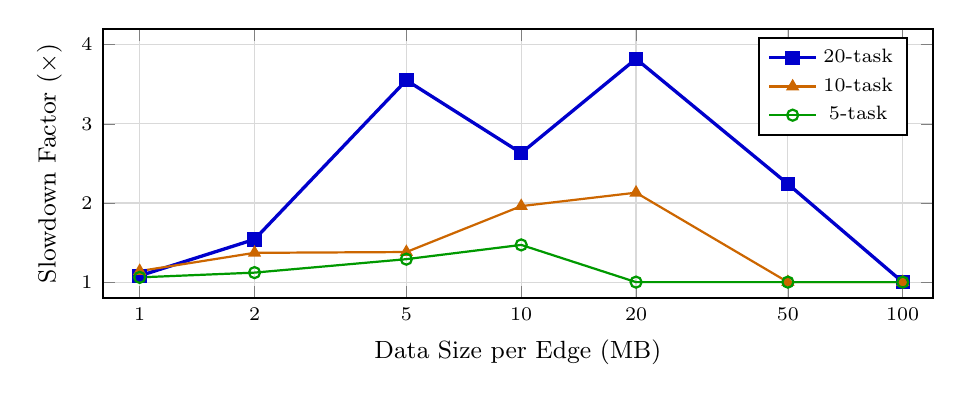
\begin{tikzpicture}
\begin{axis}[
  width=\columnwidth,
  height=5cm,
  xlabel={Data Size per Edge (MB)},
  ylabel={Slowdown Factor ($\times$)},
  xmode=log,
  xmin=0.8, xmax=120,
  ymin=0.8, ymax=4.2,
  grid=major,
  grid style={gray!30},
  thick,
  every axis label/.style={font=\small},
  tick label style={font=\scriptsize},
  legend pos=north east,
  legend style={font=\scriptsize},
  xtick={1,2,5,10,20,50,100},
  xticklabels={1,2,5,10,20,50,100},
]
\addplot[blue!80!black, very thick, mark=square*, mark size=2pt]
  coordinates {
    (1, 1.08) (2, 1.54) (5, 3.55) (10, 2.63) (20, 3.82) (50, 2.24) (100, 1.00)
  };
\addplot[orange!80!black, thick, mark=triangle*, mark size=2pt]
  coordinates {
    (1, 1.14) (2, 1.37) (5, 1.38) (10, 1.96) (20, 2.13) (50, 1.00) (100, 1.00)
  };
\addplot[green!60!black, thick, mark=o, mark size=2pt]
  coordinates {
    (1, 1.06) (2, 1.12) (5, 1.29) (10, 1.47) (20, 1.00) (50, 1.00) (100, 1.00)
  };
\legend{20-task, 10-task, 5-task}
\end{axis}
\end{tikzpicture}
\caption{Interference slowdown vs.\ data size per edge (3$\times$3 grid,
  HEFT, shortest-path).  Slowdown peaks at intermediate CCR values
  where transfers are long enough to contend but not so large that the
  scheduler collapses tasks onto one node.}
\label{fig:ccr}
\end{figure}

\subsubsection{Multi-DAG Contention}

In practice, edge computing platforms rarely service a single workflow in
isolation---multiple applications submit DAGs concurrently, and their
transfers share the same wireless medium.  To evaluate how \ncsim{}
captures this multi-tenant scenario, we inject $k \in \{1, 2, 3, 4, 5\}$
identical 5-task fork-join DAGs with 0.5\,s stagger on the 3$\times$3 grid
(HEFT, shortest-path).  Each DAG is scheduled independently, meaning that
HEFT optimizes each workflow without knowledge of the others' transfers.

\Cref{fig:multidag} shows that contention scaling is super-linear
under \texttt{csma\_bianchi}.  Without interference, $k{=}5$ DAGs
produce $2.14\times$ the makespan of $k{=}1$ ($18.0$\,s vs.\ $8.4$\,s),
reflecting the expected linear increase from staggered injection plus
queuing at compute nodes.  With interference, however, $k{=}5$ produces
$3.23\times$ the single-DAG makespan ($39.9$\,s vs.\ $12.4$\,s).  The
gap between the two curves widens with each additional DAG: the slowdown
factor grows from $1.47\times$ at $k{=}1$ to $1.70\times$ at $k{=}2$ to
$2.21\times$ at $k{=}5$, indicating a positive feedback loop.  Each
additional DAG contributes not only its own transfers to the contention
pool but also prolongs the duration of existing transfers (through reduced
effective bandwidth), which in turn increases the temporal overlap with
subsequent DAGs.  This super-linear scaling is invisible to
interference-free models, which predict near-linear growth and would
substantially underestimate the makespan of multi-tenant edge deployments.

\begin{figure}[t]
\centering
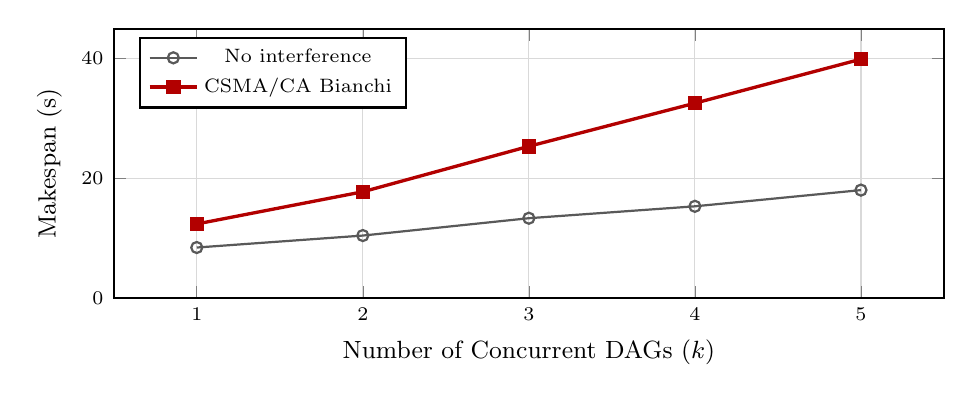
\begin{tikzpicture}
\begin{axis}[
  width=\columnwidth,
  height=5cm,
  xlabel={Number of Concurrent DAGs ($k$)},
  ylabel={Makespan (s)},
  xmin=0.5, xmax=5.5,
  ymin=0, ymax=45,
  grid=major,
  grid style={gray!30},
  thick,
  every axis label/.style={font=\small},
  tick label style={font=\scriptsize},
  legend pos=north west,
  legend style={font=\scriptsize},
  xtick={1,2,3,4,5},
]
\addplot[gray!70!black, thick, mark=o, mark size=2pt]
  coordinates {
    (1, 8.43) (2, 10.43) (3, 13.33) (4, 15.32) (5, 18.03)
  };
\addplot[red!70!black, very thick, mark=square*, mark size=2pt]
  coordinates {
    (1, 12.37) (2, 17.75) (3, 25.35) (4, 32.56) (5, 39.92)
  };
\legend{No interference, CSMA/CA Bianchi}
\end{axis}
\end{tikzpicture}
\caption{Multi-DAG makespan scaling on 3$\times$3 grid (5-task DAGs,
  HEFT, shortest-path).  Contention amplifies super-linearly: the
  gap between the curves widens from $1.47\times$ ($k{=}1$) to
  $2.21\times$ ($k{=}5$).}
\label{fig:multidag}
\end{figure}

\subsubsection{Sensitivity Summary}

\Cref{tab:sensitivity_summary} consolidates the findings across all three
sensitivity dimensions.  Taken together, these results delineate an
\emph{interference danger zone}---the conjunction of parameter settings
under which interference effects are most severe and most likely to change
scheduling conclusions.  Wireless interference has the greatest
impact---and is most likely to produce rank inversions---in environments
with moderate-to-high path loss ($n \geq 3.0$), moderate
communication-to-computation ratio (5--20\,MB payloads per edge), and
multiple concurrent workflows ($k \geq 2$).

These conditions are not exotic.  A path loss exponent of $n = 3.0$
corresponds to a typical indoor office or warehouse environment.  Data
payloads of 5--20\,MB per DAG edge are representative of computer vision
pipelines (transferring image frames between processing stages) and
sensor fusion applications (aggregating data from multiple modalities).
Multiple concurrent workflows are the norm on shared edge platforms.
In other words, the interference danger zone corresponds precisely to the
deployment scenarios that motivate edge computing research---which means
that tools ignoring interference are most unreliable in exactly the
settings where they are most needed.

\begin{table}[t]
\centering
\caption{Sensitivity analysis summary.  Each row identifies the
parameter regime where interference impact is most severe.}
\label{tab:sensitivity_summary}
\begin{tabular}{@{}llll@{}}
\toprule
\textbf{Experiment} & \textbf{Parameter} & \textbf{Danger Zone} & \textbf{Peak Effect} \\
\midrule
Path loss   & Exponent $n$    & $n \geq 3.0$      & $105\times$ at $n{=}3.5$ \\
CCR         & Data size (MB)  & 5--20\,MB          & $3.8\times$ at 20\,MB \\
Multi-DAG   & DAG count $k$   & $k \geq 2$        & $2.2\times$ gap at $k{=}5$ \\
\bottomrule
\end{tabular}
\end{table}


\subsection{Scalability}
\label{sec:scalability}

Our experiments validate \ncsim{} at scales up to 4$\times$4 grids (16
nodes, 68 links) with 20-task DAGs.  At these sizes, the Python
implementation completes in seconds on commodity hardware.  The main
computational bottlenecks are: (1)~conflict graph construction, which uses
the Bron-Kerbosch algorithm (exact for $\leq 50$ links, with a greedy
approximation fallback for larger graphs); and (2)~event queue size, which
grows with concurrent transfers.  Scaling to larger networks (e.g.,
8$\times$8 grids or 100+ node topologies) may require the greedy clique
approximation and would benefit from a compiled-language event queue, but
remains tractable for the scheduling studies \ncsim{} targets.


%% ============================================================
\section{Visualization and Tooling}
\label{sec:viz}

In order to support debugging and pedagogical use, \ncsim{} includes a
React/D3 web-based visualization frontend.  The visualization provides three
complementary views:
\begin{enumerate}[itemsep=1pt,leftmargin=*]
\item A \textbf{network topology view} that displays nodes with their compute
  capacities, links with their current bandwidths, and active transfers
  highlighted with color-coded flow indicators.
\item A \textbf{Gantt chart} showing task execution and data transfer timelines
  per node, making it possible to visually identify scheduling bottlenecks,
  idle periods, and contention-induced delays.
\item An \textbf{animated replay} with playback controls (play, pause, step,
  speed adjustment) that allows researchers to observe the dynamic evolution
  of the simulation, including the bandwidth recalculation cascades described
  in \Cref{sec:engine}.
\end{enumerate}

Simulation output is written in JSONL trace format, with one JSON object
per event, enabling integration with external analysis tools such as
pandas, matplotlib, and custom post-processing scripts.  The command-line
interface supports batch execution with configurable scheduling, routing,
and interference parameters, facilitating the automated parameter sweeps
used throughout \Cref{sec:eval}.


%% ============================================================
\section{Discussion and Limitations}
\label{sec:discussion}

In this section, we discuss the implications of our findings, the
boundaries of \ncsim{}'s modeling approach, and directions these results
suggest for future scheduler design.

\textbf{When is flow-level modeling trustworthy?}
\ncsim{}'s flow-level approach (\Cref{tab:scope}) models data transfers
as bulk flows with analytically-derived rates rather than simulating
individual packets.  This abstraction is appropriate for the workloads
studied here (10\,MB payloads per edge), where steady-state throughput
dominates and TCP slow-start transients are negligible.  For workloads
with many short transfers (e.g., sub-100\,KB control messages or
request-response patterns), the slow-start phase represents a significant
fraction of each transfer's duration, and packet-level simulation would
be warranted.  The Bianchi model further assumes saturation conditions,
meaning that every station always has a packet ready to transmit.  This
assumption overapproximates interference during periods of low load,
making our interference-aware makespans conservative upper bounds.
In practice, this means that the rank inversions and regret values we
report may be \emph{understated} relative to non-saturated conditions
where bursty traffic patterns create intermittent but intense contention.

\textbf{Scope of the experimental study.}
Our study covers three schedulers, three DAG sizes, and three grid
topologies, all with deterministic parameters (fixed seed, no stochastic
fading).  While this covers a meaningful range of conditions, the grid
topology is regular and symmetric; real deployments may have irregular
node placements that create asymmetric interference patterns.  Scaling
to 50--100 node networks is computationally feasible with \ncsim{} but
was not explored here.  Real wireless channels exhibit fading and
mobility effects that could either smooth or amplify the interference
effects we observe; we used deterministic path loss throughout to isolate
the effects of contention and hidden terminals.

\textbf{Implications for scheduler design.}
The rank inversion finding suggests that the next generation of DAG
schedulers for wireless edge computing should be \emph{interference-aware}:
the scheduler should account for wireless contention when making placement
decisions, not merely optimize the critical path assuming uncontested
bandwidth.  Our results point to several concrete design directions.
First, schedulers could query the conflict graph during placement to
estimate how many concurrent transfers a candidate placement would
create, penalizing placements that generate dense contention neighborhoods.
Second, two-phase scheduling could first compute a placement assuming
uncontested bandwidth (using HEFT or similar), then simulate the resulting
contention and iteratively reassign tasks that contribute most to
contention.  Third, schedulers could incorporate an interference
``budget'' analogous to energy budgets in sensor network scheduling,
limiting the number of concurrent cross-node transfers to keep contention
within acceptable bounds.  \ncsim{} provides the simulation infrastructure
needed to develop and evaluate such approaches.

\textbf{Implications for edge computing research.}
More broadly, the rank inversion finding carries a methodological
implication for the edge computing research community.  DAG scheduling
evaluations that assume uncontested links risk not only inaccurate
performance predictions but systematically wrong conclusions about which
algorithms are superior.  A researcher who evaluates HEFT against
round-robin on a fixed-bandwidth model would conclude that HEFT is
universally superior; our results show that this conclusion reverses
in 4 of 6 scenarios involving the 4$\times$4 grid.  \ncsim{} enables
researchers to incorporate realistic wireless modeling at low cost---a
single 108-run comparison completes in under 4 minutes---avoiding these
systematic blind spots.


%% ============================================================
\section{Conclusion and Future Work}
\label{sec:conclusion}

We presented \ncsim{}, a lightweight discrete-event simulator that bridges
the gap between heavyweight network simulators and task-centric scheduling
tools by combining DAG workflow scheduling with physically-grounded 802.11
WiFi models in a single, easy-to-use Python package.  The simulator's
modular architecture, built on six pluggable abstract base classes, enables
rapid experimentation with different scheduling algorithms, routing
strategies, and interference models.  We validated the WiFi model through
nine internal experiments (all matching analytical predictions exactly) and
external reproduction of Bianchi's published results (matching within
0.003\%), establishing both self-consistency and fidelity to the canonical
analytical framework.

The key finding enabled by \ncsim{} is that wireless interference causes
not merely inaccurate performance predictions but \emph{systematically wrong
scheduler choices}.  In a 108-run factorial comparison across three
schedulers, three network sizes, and three DAG complexities, the scheduler
that appeared optimal under an interference-free model was dominated under
realistic CSMA/CA conditions in 38.9\% of scenarios, with performance
regret reaching 484\%.  The sophisticated HEFT scheduler, which dominates
under interference-free evaluation, was outperformed by a simple round-robin
baseline in 4 of 6 large-network scenarios.  Sensitivity analyses further
revealed that interference impact exhibits sharp regime transitions with
path loss exponent, peaks at moderate communication-to-computation ratios,
and amplifies super-linearly with concurrent workflows---conditions that
characterize the wireless edge deployments that motivate this research.

These findings underscore the value of tools like \ncsim{} that make
realistic wireless modeling accessible without the computational overhead
of packet-level simulation.  We identify several specific directions for
future work: (1)~developing interference-aware scheduling heuristics that
query the conflict graph during task placement to avoid generating dense
contention neighborhoods; (2)~dynamic rescheduling that adjusts task
placements in response to observed network congestion during execution;
(3)~incorporating node mobility with time-varying topology to model
scenarios such as robotic edge computing; (4)~multi-slot node execution
to support GPU-like parallelism in heterogeneous edge deployments;
(5)~energy consumption models that account for the increased energy cost
of contention-induced retransmissions; and (6)~larger-scale cross-validation
against ns-3 packet-level simulations to characterize the fidelity of the
flow-level approximation across a wider range of traffic patterns.

The \ncsim{} simulator and all experimental configurations used in this
paper are available as open-source software to support reproducibility
and further investigation.


\bibliographystyle{IEEEtran}
\begin{thebibliography}{10}

\bibitem{shi2016edge}
W.~Shi, J.~Cao, Q.~Zhang, Y.~Li, and L.~Xu,
``Edge Computing: Vision and Challenges,''
\emph{IEEE Internet of Things Journal},
vol.~3, no.~5, pp.~637--646, Oct. 2016.

\bibitem{ns3}
{ns-3 Consortium},
``ns-3: A Discrete-Event Network Simulator,''
\url{https://www.nsnam.org/}, accessed Mar. 2026.

\bibitem{omnetpp}
A.~Varga and R.~Hornig,
``An Overview of the OMNeT++ Simulation Environment,''
in \emph{Proc. ICST SIMUTools}, 2008.

\bibitem{simgrid}
H.~Casanova, A.~Giersch, A.~Legrand, M.~Quinson, and F.~Suter,
``Versatile, Scalable, and Accurate Simulation of Distributed Applications
and Platforms,''
\emph{Journal of Parallel and Distributed Computing},
vol.~74, no.~10, pp.~2899--2917, 2014.

\bibitem{wrench}
H.~Casanova, S.~Pandey, J.~Oeth, R.~Tanaka, F.~Suter, and R.~Ferreira~da~Silva,
``WRENCH: A Framework for Simulating Workflow Management Systems,''
in \emph{Proc. WORKS Workshop}, 2018, pp.~74--85.

\bibitem{cloudsim}
R.~N.~Calheiros, R.~Ranjan, A.~Beloglazov, C.~A.~F.~De~Rose, and R.~Buyya,
``CloudSim: A Toolkit for Modeling and Simulation of Cloud Computing
Environments and Evaluation of Resource Provisioning Algorithms,''
\emph{Software: Practice and Experience},
vol.~41, no.~1, pp.~23--50, 2011.

\bibitem{ifogsim}
H.~Gupta, A.~Vahid~Dastjerdi, S.~K.~Ghosh, and R.~Buyya,
``iFogSim: A Toolkit for Modeling and Simulation of Resource Management
Techniques in the Internet of Things, Edge and Fog Computing Environments,''
\emph{Software: Practice and Experience},
vol.~47, no.~9, pp.~1275--1296, 2017.

\bibitem{edgecloudsim}
C.~Sonmez, A.~Ozgovde, and C.~Ersoy,
``EdgeCloudSim: An Environment for Performance Evaluation of Edge Computing
Systems,''
\emph{Transactions on Emerging Telecommunications Technologies},
vol.~29, no.~11, e3493, 2018.

\bibitem{bianchi2000}
G.~Bianchi,
``Performance Analysis of the IEEE 802.11 Distributed Coordination Function,''
\emph{IEEE Journal on Selected Areas in Communications},
vol.~18, no.~3, pp.~535--547, Mar. 2000.

\bibitem{heft}
H.~Topcuoglu, S.~Hariri, and M.-Y.~Wu,
``Performance-Effective and Low-Complexity Task Scheduling for Heterogeneous
Computing,''
\emph{IEEE Trans.\ Parallel Distrib.\ Syst.},
vol.~13, no.~3, pp.~260--274, 2002.

\end{thebibliography}

\end{document}
